%! Author = mackesmilian
%! Date = 01.11.21

% Preamble
\documentclass[11pt]{article}
\usepackage{graphicx}
\usepackage{xr}
\usepackage[english]{babel}
\usepackage[style=apa]{biblatex}
\usepackage{titlesec}
\usepackage{tocloft}
\usepackage{fancyhdr}
\usepackage{chngcntr}
\usepackage{float}
\usepackage{listings}
\usepackage{xcolor}
\usepackage[T1]{fontenc}
\usepackage[margin=3cm]{geometry}
\usepackage[acronym]{glossaries}
\usepackage{caption}
\captionsetup{justification=raggedright,singlelinecheck=false, format=plain, font=small, labelfont=bf}
\addbibresource{main.bib}
\usepackage{helvet}
\renewcommand{\familydefault}{\sfdefault}
\usepackage{csquotes}
\graphicspath{ {/home/mackesmilian/Documents/FH/BACC/bachelorarbeit/src/images/} }
\title{
        {Development and Deployment of Web Applications as Installable Desktop Applications Using
    Electron Framework}\\
    {\large FH Campus 02}\\
}
\author{Maximilian Martin Wolf}
\date{30 October 2021}
\definecolor{codegreen}{rgb}{0,0.6,0}
\definecolor{codegray}{rgb}{0.5,0.5,0.5}
\definecolor{codepurple}{rgb}{0.58,0,0.82}
\definecolor{backcolour}{rgb}{0.95,0.95,0.92}

\lstdefinestyle{mystyle}{
    backgroundcolor=\color{backcolour},   
    commentstyle=\color{codegreen},
    keywordstyle=\color{magenta},
    numberstyle=\tiny\color{codegray},
    stringstyle=\color{codepurple},
    basicstyle=\ttfamily\footnotesize,
    breakatwhitespace=false,         
    breaklines=true,                 
    captionpos=b,                    
    keepspaces=true,                 
    numbers=left,                    
    numbersep=5pt,                  
    showspaces=false,                
    showstringspaces=false,
    showtabs=false,                  
    tabsize=2
}

\lstset{style=mystyle}
\renewcommand*\glspostdescription{\dotfill}
\makenoidxglossaries
\newacronym{saas}{SaaS}{Software as as Service}
\newacronym{tls}{TLS}{Thread Local Storage}
\newacronym{npm}{npm}{Node Package Manager}
\newacronym{deb}{deb}{Debian Package}
\newacronym{poc}{POC}{Proof-of-Concept}
\newacronym{lts}{LTS}{Long Term Support}
\newacronym{crud}{CRUD}{Create, Read, Update, and Delete}

% Turn on the style
\pagestyle{fancy}
% Clear the header and footer
\fancyhead{}
\fancyfoot{}
% Set the right side of the footer to be the page number
\fancyfoot[R]{\thepage}
\renewcommand{\headrulewidth}{0pt} % to remove the rules
\renewcommand{\footrulewidth}{0pt} % to remove the rules

\AtBeginDocument{%
\renewcommand{\listfigurename}{LIST OF FIGURES}
}
\renewcommand{\cfttoctitlefont}{\normalfont\Large\bfseries\MakeUppercase}


\renewcommand{\cftsecafterpnum}{\vspace{20pt}}
\renewcommand{\cftsecdotsep}{1}
\renewcommand{\cftsubsecdotsep}{1}
\renewcommand{\cftsubsubsecdotsep}{1}
\setlength{\cftbeforesecskip}{20pt}
\setlength\cftsecnumwidth{35pt}
\setlength\cftsubsecnumwidth{35pt}
\setlength{\cftsecindent}{0pt}% Remove indent for \section
\setlength{\cftsubsecindent}{0pt}% Remove indent for \subsection
\setlength{\cftsubsubsecindent}{0pt}% Remove indent for \subsubsection

\makeatletter
\patchcmd{\l@section}{#1}{\MakeUppercase{#1}}{}{}
\makeatother

\counterwithin{figure}{section}
\renewcommand\thefigure{\thesection-\arabic{figure}}

% Document
\begin{document}

    \titleformat{\section}{\bfseries\sffamily\large\MakeUppercase}{\thesection}{0pt}{\quad}{}%
    \titlespacing{\section}{20pt}{*4}{*1.5}

    \pagenumbering{Roman}
    %\pagestyle{plain}

    \maketitle
    \clearpage

    \section*{Ehrenwörtliche Erklärung}\label{sec:ehrenwort}
    Ich erkläre ehrenwörtlich, dass ich die vorliegende Arbeit 
selbstständig und ohne fremde Hilfe verfasst, andere als 
die angegebenen Quellen nicht benützt und die benutzten 
Quellen wörtlich zitiert sowie inhaltlich entnommene Stellen 
als solche kenntlich gemacht habe.\paragraph*{}

I hereby declare that I am the sole author of this work; 
no assistance other than that permitted has been used and 
all quotes and concepts taken from unpublished sources, 
published literature or the internet in wording or in basic 
content have been identified by footnotes or with precise 
source citations.\paragraph*{}
.................................\paragraph*{}
Unterschrift
    \clearpage
    \section*{Kurzfassung}\label{sec:kurzfassung}
    Web Applikationen haben über die letzten Jahre einen Zuwachs 
in Popularität und Komplexität erfahren was zu einem regelrechten
Ruck von Desktopapplikationen zu Web Applikationen geführt hat. 
Mehr Internetnutzer*innen, schnellere Internetgeschwindigkeiten 
und finanzielle Gründe haben zu diesem Wechsel beigesteuert. 
Dadurch stellt sich natürlich die Frage ob dieser Weg der 
einzige ist um Applikationen an Nutzer*innen zu bringen. 
Schließlich setzen Web Applikationen beispielsweise eine stabile 
Internetverbindung vor.
Um diese Probleme zu umgehen sind einige Framworks entstanden, die
versprechen, solche Nachteile von Web Applikationen zu beseitigen. 
Eines solcher Framworks ist Electron, welches Entwickler*innen
ermöglicht, native Desktopapplikationen ausschließlich mit 
Webtechnologien wie JavaScript, HTML und CSS zu entwickeln.
Das Ziel dieser Arbeit ist eine Evaluierung dieses Framworks
mit Blick auf Vor- und Nachteile welche von Entwickler*innen
in Betracht genommen werden könen, wenn Electron zum Einsatz kommen würde. 
Um diese Lücke zu schließen wurde eine Fallstudie durchgeführt 
die den Entwicklungsprozess mit Electron untersucht.
Daraus resultierend wurden Vor- und Nachteile identifiziert 
sowie Empfehlungen für Organsationen und Entwickler*innen formuliert, 
worauf bem Einsatz von Electron geachtet werden kann. 
Für künftige Forschungsarbeiten bezüglich Electron - oder auch anderen
vergleichbaren Frameworks - werden weitere relevante Problemstellungen
identifiziert wie zum Beispiel die Frage inwiefern sich Electron in 
einen produktiven Entwicklungsprozess einbinden lässt und welche 
Überlegungen in Bezug auf Wartung, Versionierung und Weiterentwicklung
in einem unternehmerischen Kontext relevant sind.
    \clearpage
    \section*{Abstract}\label{sec:abstract}
    Web applications have been gaining in popularity and complexity
over the recent years and have resulted in a de-facto move from 
the desktop to the web browser. 
More internet users, faster connection speeds, and other reasons
such as financial ones have all contributed to this rise in 
popularity of web apps. 
However one can ask themselves if this really is the only way 
forward for bringin applications to users. 
After all, relying on a constant internet connection is not 
always a guarantee, for instance.
To overcome this issue several frameworks have been developed 
which claim to overcome this hurdle by allowing web developers 
to use their expertise and experience to create desktop 
applications. 
One of such solutions is Electron, a framework promising to 
enable creating native desktop applications using only web 
technologies such as JavaScript, HTML, and CSS. 
The goal of this thesis is therefore to evaluate how Electron
achieves this and what advantages and disadvantages developers 
need to take into account.
To find conclusive answers to this issue a case study was conducted which shows the 
process of developing such an application from start to finish. 
Resulting from this case study considerations were defined which developers 
and organisations alike may take into account when deciding upon 
using Electron. 
This has also raised relevant questions to be answered in the future
such clearly quantifying how much extra work is needed for Electron 
and how Electron works in a productive environment in regards to 
maintenance, versioning and further development. 
    \clearpage

    \tableofcontents
    \clearpage

    \titleformat{\section}{\bfseries\sffamily\large\MakeUppercase}{\thesection}{0pt}{\hspace{9cm}}{}%
    \titlespacing{\section}{20pt}{*4}{*1.5}

    \pagenumbering{arabic} 
    \setcounter{page}{6}

    \section{Introduction}\label{sec:introduction}
    \setcounter{tocdepth}{3}
    In December 2012 software engineer Cheng Zhao joined GitHub's team, having previously worked for Intel developing
node-webkit, with the task of porting the Atom editor from using Chromium Embedded Framework to node-webkit.
Node-webkit being a Node.js module developed by Roger Wang which combined the browser engine used by Chromium - WebKit - 
with Node.js, making Node.js modules accessible from JavaScript code running inside a web page. \parencite{jensen2017}\paragraph{}

Porting to node-webkit proved difficult, so GitHub abandoned that approach, and it was decided that a new native shell
for Atom would be created.
Said shell was dubbed \emph{Atom Shell} and after development was finished and the Atom editor was open sourced
by GitHub, Atom Shell soon followed suit and was renamed to \emph{Electron}.
Initially developed as a way to deliver an editor, numerous widely known applications like Slack, Discord and Visual
Studio have started using Electron to develop and deliver their desktop applications.\parencite{electronDocs}
But what exactly is Electron?\paragraph{}

    \subsection{What Is Electron?}\label{subsec:what-is-electron}
    In December 2012 software engineer Cheng Zhao joined GitHub's team, having previously worked for Intel developing
node-webkit, with the task of porting the Atom editor from using Chromium Embedded Framework to node-webkit.
Node-webkit being a Node.js module developed by Roger Wang which combined the browser engine used by Chromium - WebKit - 
with Node.js, making Node.js modules accessible from JavaScript code running inside a web page. \parencite{jensen2017}\paragraph{}

Porting to node-webkit proved difficult, so GitHub abandoned that approach, and it was decided that a new native shell
for Atom would be created.
Said shell was dubbed \emph{Atom Shell} and after development was finished and the Atom editor was open sourced
by GitHub, Atom Shell soon followed suit and was renamed to \emph{Electron}.
Initially developed as a way to deliver an editor, numerous widely known applications like Slack, Discord and Visual
Studio have started using Electron to develop and deliver their desktop applications.\parencite{electronDocs}
But what exactly is Electron?\paragraph{}
Electron is a framework which allows for the development of cross-platform desktop applications using only popular 
web programming languages like HTML, CSS and JavaScript. 
While the advantages will be discussed in detail in the next chapter \emph{Why Use Electron?}, the appeal to developers
is obvious: Maintaining one codebase while being able to deliver the app to all desktop operating systems.\paragraph{}
Now, as described previously the Electron framework serves the same purpose as node-webkit (later renamed to NW.js), but
their approaches do differ in certain ways: \parencite{jensen2017}\par
\begin{figure}[ht]
    \label{fig:el-architecture}
    \caption{A simplified representation of Electron's architecture. \parencite{jensen2017}}
    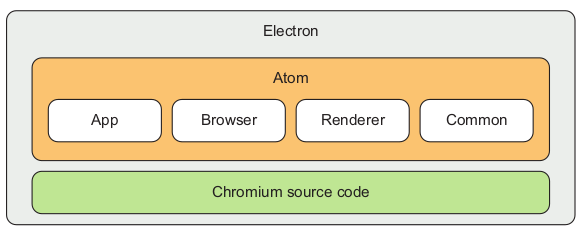
\includegraphics[width=\textwidth]{electron-architecture}
\end{figure}
Without going into detail on how NW.js works, Electron and NW.js share some architectural similarities.
However, there are some differences in how Electron combines Node.js with Chromium.\paragraph{}
Architecturally, Electron places an emphasis on strict separation from Chromium source code, ass seen in figure \ref{fig:el-architecture}.
This looser integration allows for easier updates to the Chromium part of the source code, whereas with NW.js Chromium
is patched to allow for Node.js and Chromium to use a shared Javascript state. \parencite{jensen2017}\par
On the other hand, this means that Electron has separate JavaScript contexts: A \emph{main} process which starts running
with the app window and a \emph{renderer} process for each individual window.
Any sharing of state between these contexts, or simply put between the front- and back-end, has to pass through the
\emph{icpMain} and \emph{icpRenderer} modules.
This means that each JavaScript context is kept separate but data can be explicitly shared, allowing for greater control
over what state exists in which app window. \parencite{jensen2017}\paragraph{}
Electron itself (the part without Chromium) is made up of for different components: App, Browser, Renderer and Common.
\textbf{App} contains code written in C++ and Objective-C++ responsible for loading Node.js and Chromium's content module.
The \textbf{browser} folder contains code which handles interactions with the front-end.
This is to say functionality such as loading the JavaScript engine, interacting with the UI and binding operating system
specific modules.
As for \textbf{renderer}, this component handles the different renderer processes.
Because Chromium works by running each tab as an individual process, as to not crash the entire browser should one
tab become unresponsive, each application window in Electron runs as its own process.
\textbf{Common} contains code which is used by both the main and renderer processes for running the application.
Among other things this folder also contains the integration of Node.js' event loop with Chromium's event loop. \parencite{jensen2017}\paragraph{}


    \subsection{Why Use Electron?}\label{subsec:why-use-electron}
    Now the next obvious question is why a framework such as Electron is needed at all.
After all, it is "just" a way to have desktop applications developed using HTML, CSS and JavaScript.
So why not just develop native desktop applications or traditional web applications depending on the use case?
To answer this one has to examine the bigger picture:\paragraph{}
Over the past decade it seems as though software pricing has moved from perpetual licenses towards subscription-based
models.
If one examines the data regarding end-user spending on cloud applications it is clear that the
\emph{Software as a Service} (SaaS) model has grown considerably in revenue and is projected to do so in the future:
The worldwide end user spending for Software as a Service has increased from 31.4 billion US Dollars in 2015 to 120
billion US Dollars in 2020.
It is projected this growth will progress with spending reaching 171.9 billion dollars in 2022. \parencite{gartner2021}\paragraph{}
Furthermore, \textcite{gartner2021} forecasts that by 2026, cloud spending will exceed 45\% of all enterprise IT spending, up from
17\% in 2021.
This impressive growth can be attributed to two reasons.
Reasons either technical and/or financial in nature.
One financial benefit of SaaS is economies of scale:
By hosting the application centrally and by extension aggregating users together, providers can benefit financially from
leveraging economies of scale.
At the simple end, this means benefiting from volume pricing on hardware such as data centers, servers, space and so on.
Taking this idea further, SaaS providers can also cut costs by sharing hardware across their customers.
It is not cost-effective to use one machine for each customer, instead resources should be shared and dynamically
allocated on-demand to each customer's needs.
Similarly, as user count increases, the cost of adding on single user decreases.
These and other reasons are a big financial motivator for providers of software to switch to the SaaS model.\paragraph{}
However, technological reasons play a large role as well.
According to \textcite{jacobs2005} the ever-increasing maturity of the Web is a major contributor for the rise in popularity of
SaaS.\par
Browsers are significantly more powerful than ever. 
The \emph{browser wars} of the mid-to-late nineties started with Microsoft and Netscape outdoing each other with
new features, faster and overall better browsers leading to significant leaps in browser technology. \parencite{mozilla2021,jensen2017}\paragraph{}
Furthermore, internet access is more widespread than ever.
In the United States, the number of internet users rose from 229,91 million in 2010 to 302,28 million in 2021,
which constitutes a 31\% increase.\par
\begin{figure}[H]
    \centering
    \label{fig:num-of-internet-users}
    \caption{Number of internet users in the US from 2010 to 2025. \parencite{statista2021}}
    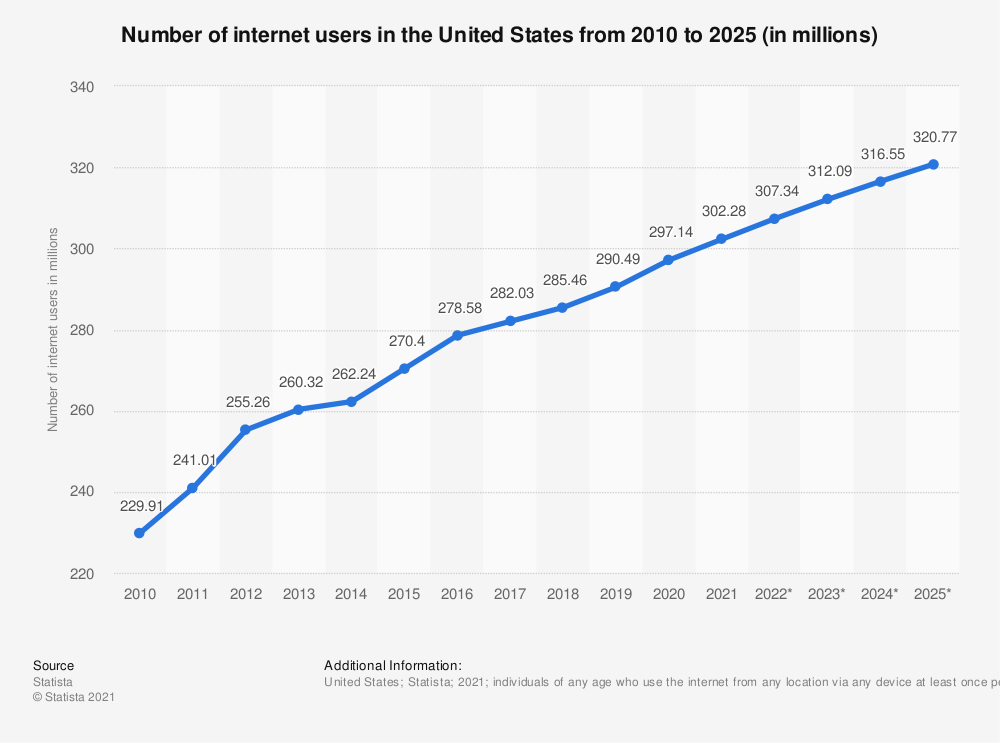
\includegraphics[width=0.8\textwidth]{number-of-internet-users}
\end{figure}
And not only have the number of internet users risen over the past eleven years, the average connection speed increased as well
over the same time period:
\begin{figure}[H]
    \centering
    \label{fig:internet-speed}
    \caption{Average internet connection speed in the US 2007-2017. \parencite{akamai2017}}
    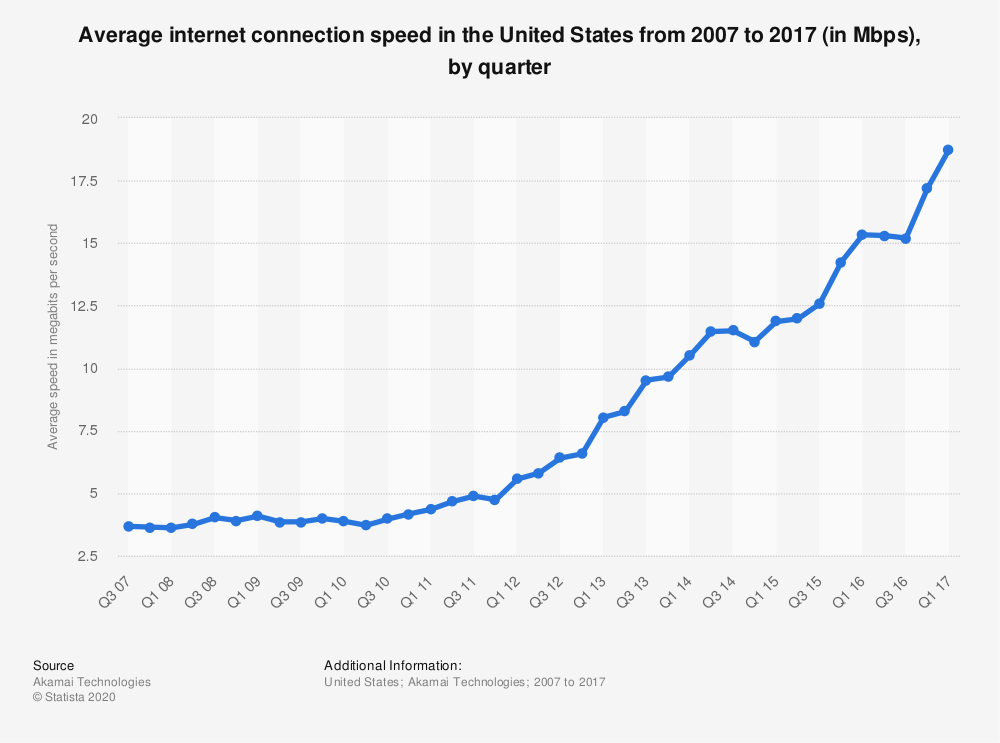
\includegraphics[width=0.8\textwidth]{internet-connection-speed}
\end{figure}
As seen above, from Q3 2017 to Q1 2017, average internet speeds across the US rose by 410\%.
This allowed for much more elaborate websites where larger amounts of data have to be downloaded.
Moreover, the number of robust frameworks for web development (be it front-end or back-end), make creating a complex web application easier
than ever before.
However, while this explains why SaaS is often the billing model of choice, it doesn't fully explain why specifically web applications
have risen in popularity. \parencite{statista2021}\par
After all, SaaS can also be delivered as a Desktop Application, as seen with the Adobe Creative Suite for example. \parencite{adobe2021}\par
To answer this, one should examine how desktop applications and web applications differ in more detail.



    \subsubsection{Desktop Applications}\label{subsubsec:desktop-applications}
    Desktop applications used to be the standard way of delivering software to the end user.
Users had to go to a store, buy a CD-ROM, check the system requirements and install the software 
on their machine.
This does of course come with a number of benefits over web applications.\par
One advantage is that desktop applications aren't reliant on an internet connection.
Web applications obviously fail here, as their are accessed over the internet.
Furthermore, this reliance on an internet connection leads to more issues when the application
is very feature-rich and/or has to support large files. 
An image editing software as a web application for example can run into limitations when being
used with high-resolution images. 
Similarly, desktop applications start instantly without having to download resources over the 
internet. 
In such cases, desktop applications have an edge over comparable web applications.\cite{jensen2017}\par
There of course also benefits to using desktop applications from a developer's perspective.
As a developer, one does not have to worry about users accessing their web applications over different web browsers 
as the choice of browser is at the user's discretion. 
This means not having to consider how different browser interpret CSS, for example. 
Another benefit is the fact of tighter integration with the user's OS.
Browser security limits the use of hardware and can lead to challenges for certain use cases.\cite{jensen2017}\par
Moreover, another benefit of having an installable desktop application is not having to continuously support all the necessary infrastructure.
There simply is no need to run servers, databases and such when the application is locally installed on each user's machine.\cite{jensen2017}


    \subsubsection{Web Applications}\label{subsubsec:web-applications}
    \externaldocument{main.tex}
In contrast to desktop applications, the relatively low barrier for entry thanks to the easy of learning
the basics of HTML, CSS and JavaScript in web development makes it much easier for developers to create complex web applications. 
With the amount of open source frameworks developers of web apps have a large selection of different solutions to fit
their specific use case.
Also, package managers like npm offer a large selection of readily available, well established packages for developers to use
and enhance their projects.\paragraph{}
Another big advantage of web applications is that they are platform-independent. 
A web application can be reached on any reasonably modern device which runs a web browser.
There is no need to create a separate version for all the operating system one wants to support and 
websites can also easily be accessed on mobile devices.\paragraph{}
As described in the previous chapter \ref{subsubsec:desktop-applications}, web applications need continuously running infrastructure such as
web servers and databases. 
While this constitutes a disadvantage, it also comes with a big benefit for developers, as they can strictly control which version 
a client uses.
Furthermore, the access to real-world data in said databases makes reproducing bugs much simpler. \parencite{jacobs2005}

    \subsubsection{Electron as a Solution}\label{subsubsec:electron-as-solution}
    \externaldocument{main.tex}
However, web applications do come with disadvantages. 
As described in \ref{subsubsec:desktop-applications} web apps have their shortcomings such as 
browser security preventing access to a user's file system or having no access as soon as the internet connection
fails.\paragraph{}
This is where frameworks such as Electron manage to strike the near-perfect balance between desktop application and web app.
For instance the drawback of not having access to a user's PC's file system does not apply to applications 
developed using Electron, as the npm module \emph{osenv} can for example retrieve the user's home folder among 
other environment settings. \parencite{osenv}\paragraph{}
Additionally, the disadvantage of having to consider different browsers (and versions thereof) are a non-issue
with electron because Electron uses Chromium as outlined in \ref{subsec:what-is-electron}. 
Furthermore, internet access is not a requirement with Electron which means applications can have some offline
functionality as opposed to web apps.\par
These are some features and advantages of Electron, though not an exhaustive list. \parencite{electronDocs}\paragraph{}
Ultimately, it is at the developer's discretion which form of software to use.
Native desktop applications, web applications or applications developed using frameworks such as Electron 
all have advantages and disadvantages and it is important to consider
which solution fits an application's and/or user's needs best.\paragraph{}
During the course of this bachelor thesis, Electron will be evaluated as a framework for developing desktop applications
by implementing an example project. 
The aforementioned considerations and points will be examined in development of said application and 
finally an evaluation will be made on how effective of an alternative to web applications Electron is 
and whether the biggest shortfalls of web applications can be eliminated or mitigated by 
using Electron.
    \clearpage

    \section{Case Study}\label{sec:method}
    \externaldocument{main.tex}
Using the Design Science approach \parencite{VaishnaviVijayKuechler} an artifact will be developed using Electron.
Said artifact is a proof-of-concept application which will be used to gauge whether Electron would be an effective
solution in this specific and other different use cases. \paragraph{}
The application to be developed will be developed similarly to an already existing application.
Said application is a time keeping app developed by and used by Comm-Unity GmbH, a company specialising in e-government
software.
This web app is used by all employees to record the time worked based on factors such as customers, projects and other
internal, domain-specific aspects.\paragraph{}
The existing application is a web-only application developed using Vaadin 
(Vaadin is a server-side Java-only framework for web development)\parencite{vaadinDocs}.
By developing a similar application using Electron one can directly judge where the advantages and 
disadvantages of Electron lie. 
    \externaldocument{main.tex}
As mentioned before the intention of the application is to facilitate efficient time keeping 
for employees of Comm-Unity EDV GmbH. 
As with any business-oriented time keeping program it is central to be able to book 
time worked on specific data points not only to be able to bill customers correctly but also to 
create a clearer picture of which project and/or customer require what amount of attention by 
employees.
In this specific proof-of-concept we will limit said data points to customers and projects.\paragraph{}
These can be easily extended customised depending on domain-specific requirements and needs but as far 
as this example goes, a generalised approach is sufficient and also required as to extrapolate results 
on other use cases.\paragraph{}
The below described requirements have been deducted from decades long experience within the company in question.
As a comparable application has been in use for 20 years, users of this tool and engineers who were involved
in designing the legacy application have an extensive knowledge of what improvements were required.
These improvements were then defined as new features and continuously re-evaluated throughout development.
These re-evaluation cycles used input from software engineers with extensive company specific knowledge and
experienced users.
Therefore the requirements for the artifact created and discussed within this thesis were adopted from the existing
application developed for Comm-Unity EDV GmbH.\paragraph{}
The application will be structured into four different views. 
The main view shows a list of entries which each represent a data point.
Said data point has a start and end time a project and customer are assigned to each entry. 
As the number of customers and projects increases over time it becomes increasingly difficult for 
employees to quickly find the correct values to attribute their entries to.
To make this easier to use users can create templates which limit the possible data points one can
choose.\paragraph{}
The second view is the so called template view which shows a list of the aforementioned templates.
Users can create, update and delete templates which each have a unique ID, a name and a list of projects 
and customers.\paragraph{}
The third view is an overview of customers, which can be created, updated and removed. 
Each customer is comprised of a name and an address.\paragraph{}
The fourth view is similar to the customers view but represents an overview of projects, which 
can also be created, updated and removed.
Each project contains a name and whether said project is active or not.\paragraph{}

    \externaldocument{main.tex}
The application can be split into three distinct parts from a technological/architectural point of view:
\begin{itemize}
  \item The back-end API used to fetch and save data.
  \item The front-end part using Angular\parencite{angularDocs}.
  \item The Electron part used to deploy the application and to offer offline functionality.
\end{itemize}
The back-end uses a MongoDB \parencite{mongoDocs} database to persist data. 
The decision to choose MongoDB was taken because of the use
case: A time keeping application needs to be highly flexible.
Entities such as projects and customers and the general company structure and therefore evolving requirements can change over time, 
possibly necessitating a different database structure. 
Due to MongoDB being a No-SQL database based on a JSON-like document structure, future changes regarding documents (which are analogous to tables 
in relational databases) require no changes to the database itself.
Such flexibility would greatly increase the future proofing of such an application.\paragraph{}
The back-end logic is developed in Python and uses the Flask framework \parencite{flaskDocs} for handling
requests from the front-end.
As mentioned previously for each entity (project, customer, template, and entry) there is business
logic to support create, update, and remove operations.\paragraph{}
The front-end uses Angular \parencite{angularDocs} and Angular Material \parencite{angularMaterialDocs}.
Angular was chosen as it is a very popular framework for single page applications and furthermore,
it makes it easy to develop re-usable UI components.
As for the components library, Angular Material was used because of its ease of use and well-known design, 
meaning users can easily adjust to the new user interface.
\begin{figure}[H]
  \centering
  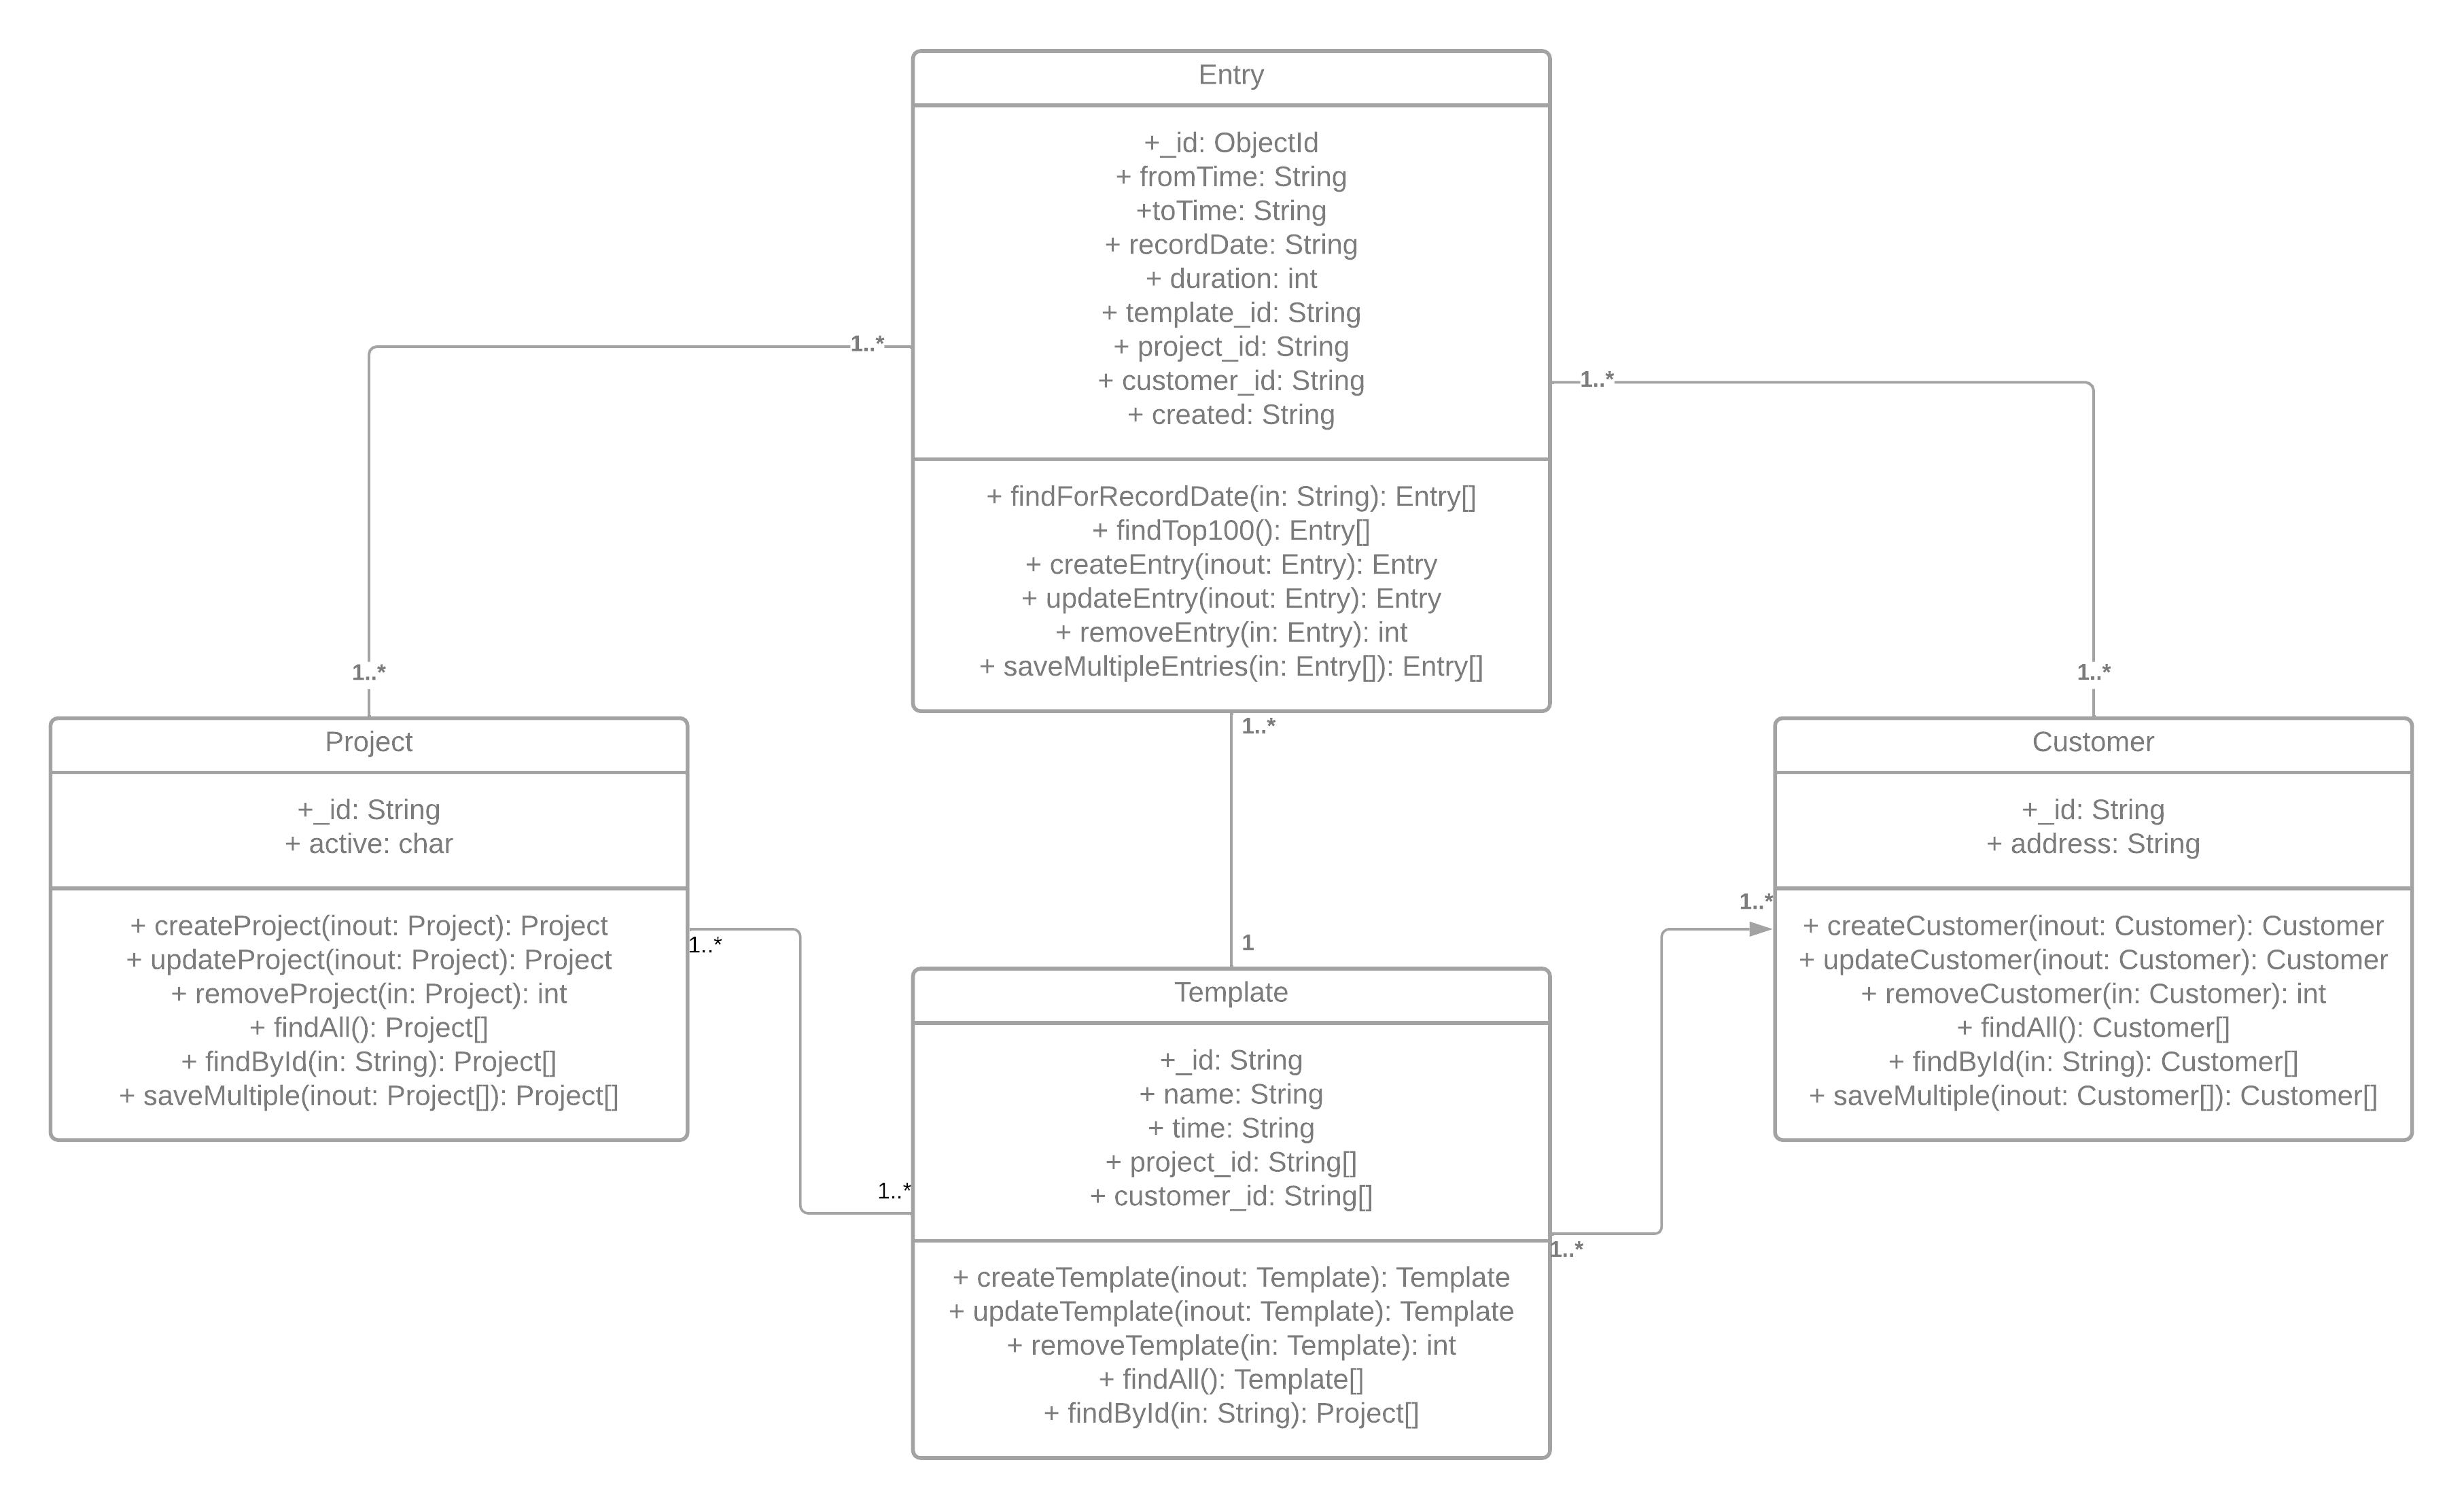
\includegraphics[width=1\textwidth]{pze-class-diagram}
  \caption{A class diagram representing all entities, relationships and operations.}
  \label{fig:pze-class-diagram}
\end{figure}
As seen in the figure above, all entities have similar operations and relationships. 
Each can be created, updated, and removed.
Furthermore, each offers an operation to fetch an entity based on its ID, as those are retrieved on-demand and not 
fetched eagerly.
Additionally, the Entry entity contains an operation to fetch the 100 latest entries (ordered by their recordDate attribute) in
order to return data for a local backup on each user's machine.
As the number of entries will grow once this is in use it is neither practical nor sensible to fetch all records from the database
just to make offline usage possible. 
Another unique operation of the Entry entity is fetching Entries based on their recordDate attribute. 
This is necessary as users view entries on a per-day basis.\paragraph{}
Entry, Project and Customer entities each contain an operation which allows for the creation of multiple of their respective entities.
This is to facilitate the offline functionality where users can create entities while not connected to the back-end API. 
Said entities are saved locally and once connection is restored, they are posted to the back-end and persisted.\paragraph{}
An instance of a template always references at least one customer and project, meaning that each entry which always references exactly one template 
always references at least one project and customer. 
One template can of course be referenced by multiple entries and one template can reference multiple project and vice-versa.
On the database level, a template holds an array of project and customer IDs as references.
The IDs of customer and project entities are a string representation of their given name as those have to be unique.\paragraph{}
\begin{figure}[H]
  \centering
  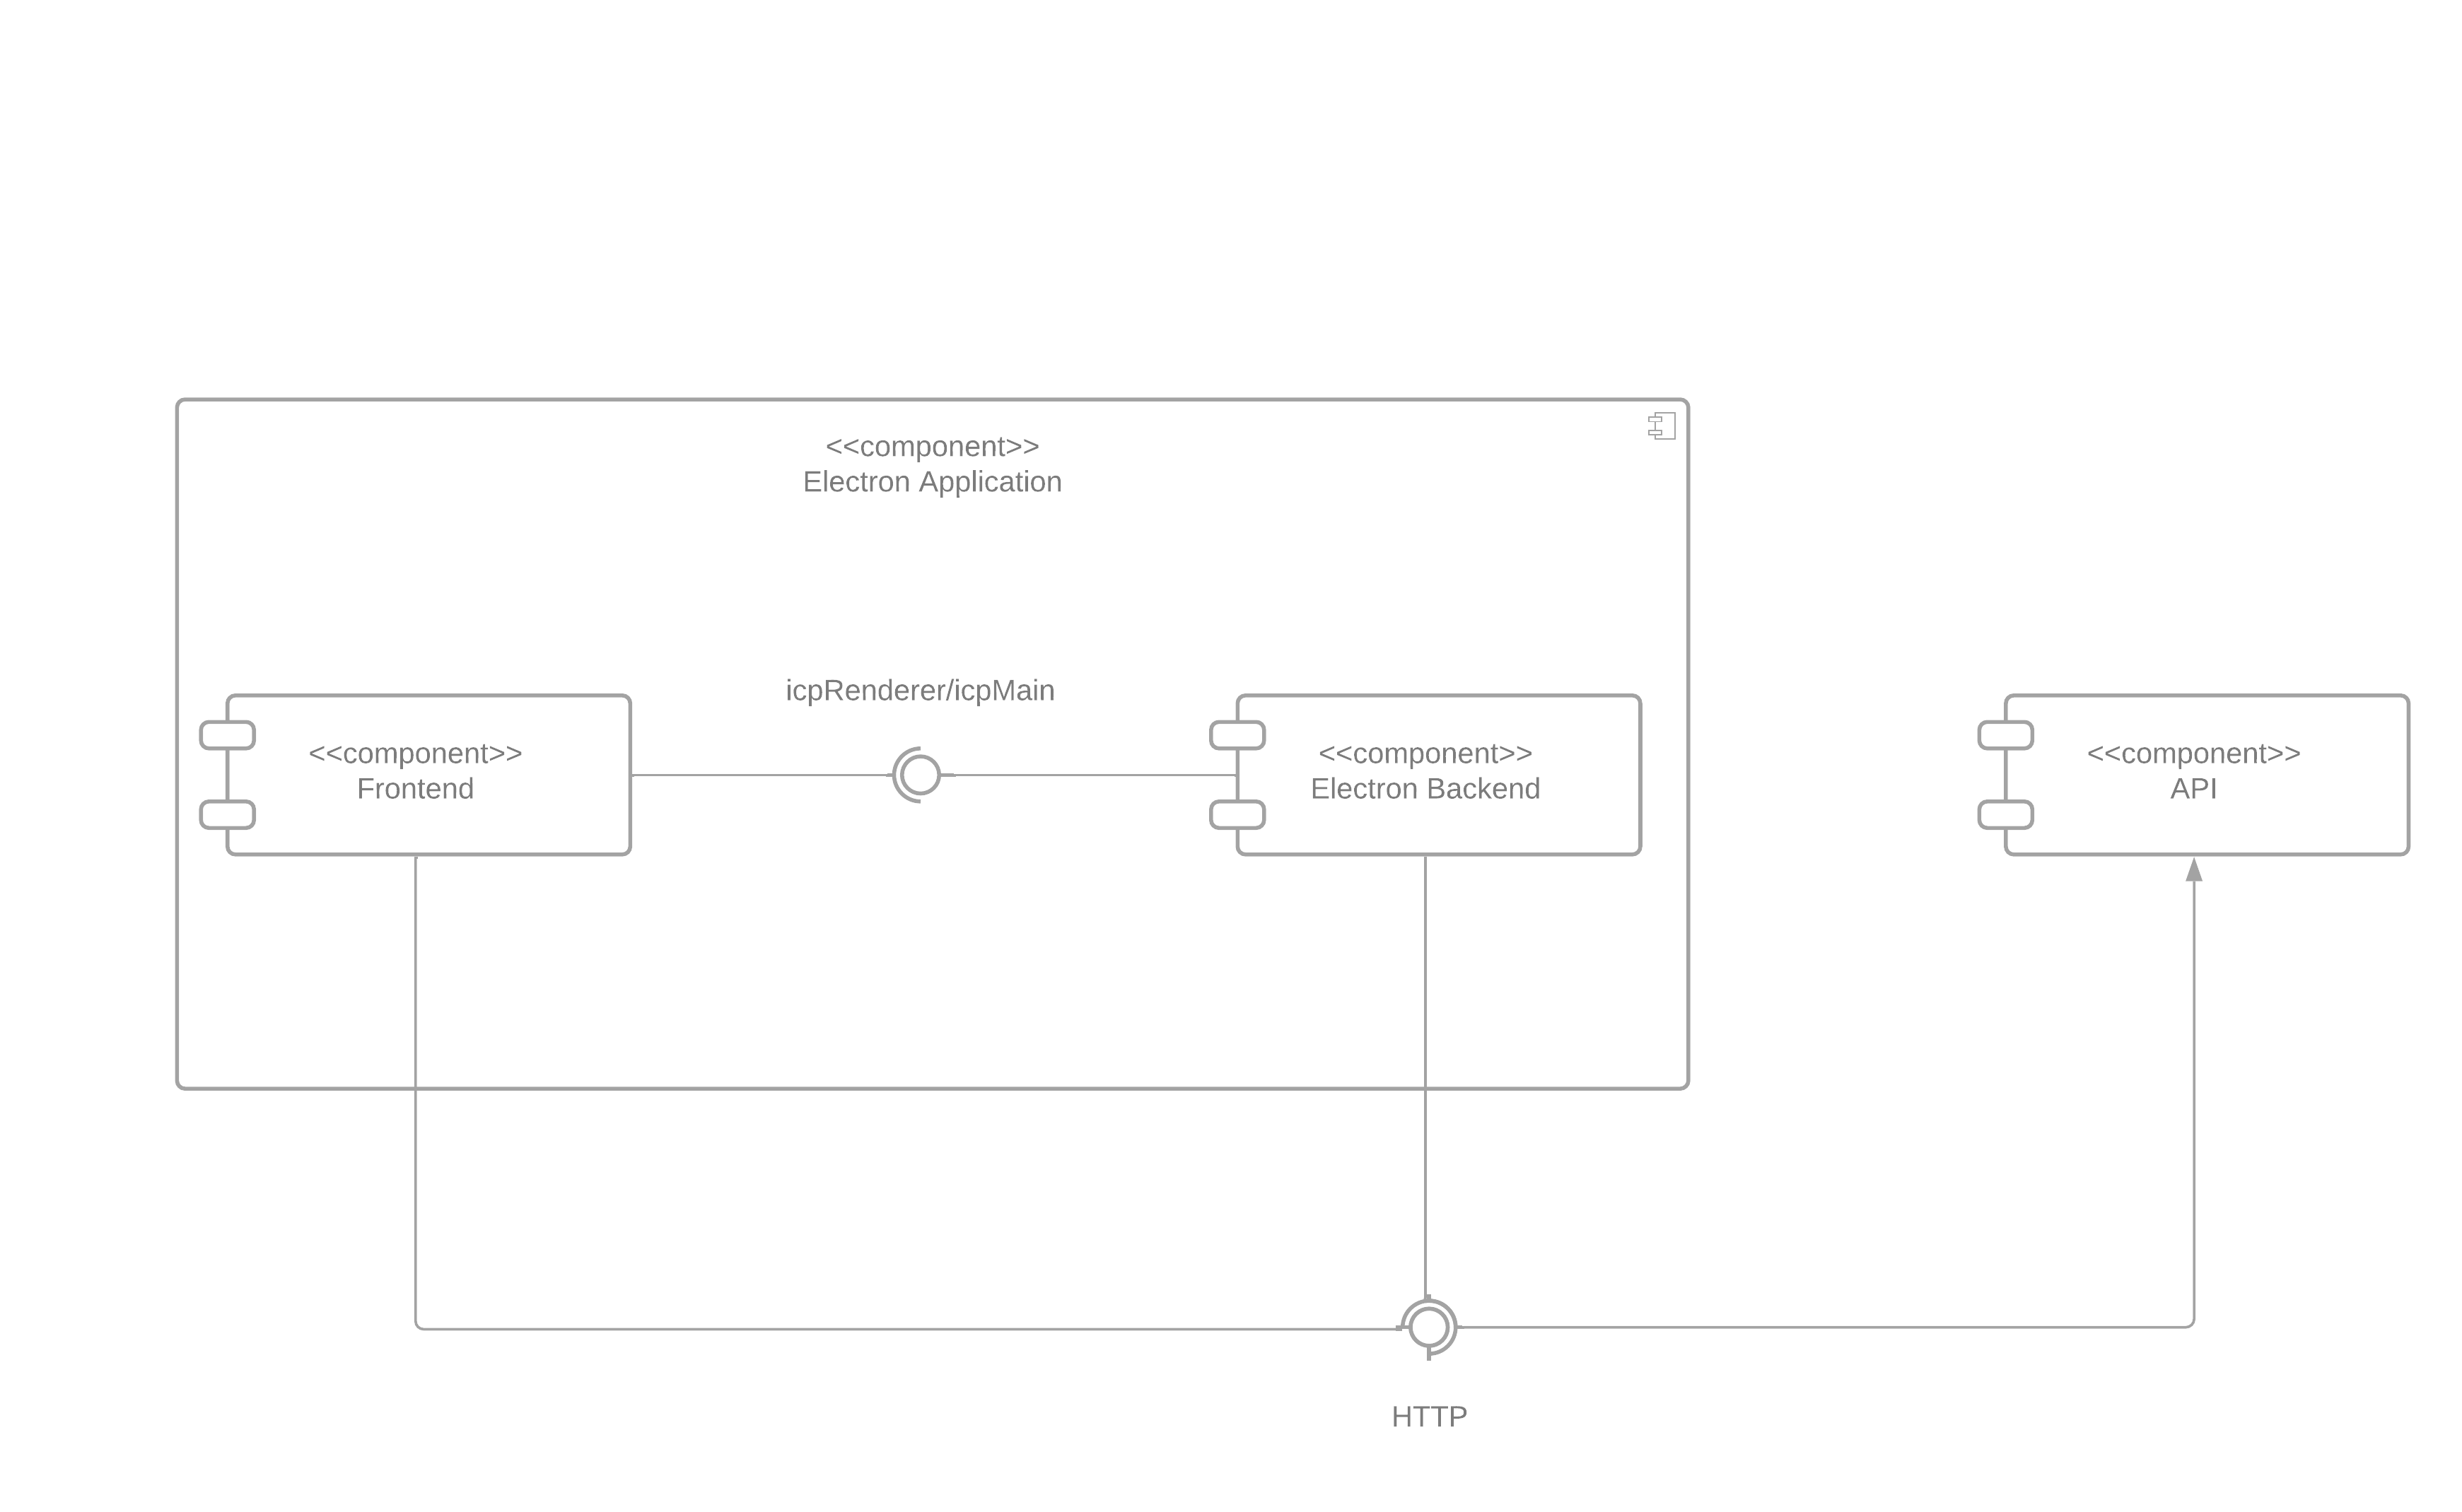
\includegraphics[width=1\textwidth]{pze-component-diagram}
  \caption{A schematic overview of the application components, simplified.}
  \label{fig:pze-component-diagram}
\end{figure}
The above figure shows a simplified overview of the applications's components. 
For the sake of illustration some implementation details have been omitted, such as the details of the database implementation in the 
back-end API.
In essence there are two ways the front-end can communicate with a data source:
Either over HTTP requests with directly the back-end or through the icpMain and icpRenderer processes with the Electron-provided back-end.
The details of this implementation will be discussed in a later chapter. 
To further illustrate the interaction between the application's components, see the following sequence diagram which illustrates
the workflow of creating an entry. 
\begin{figure}[H]
  \centering
  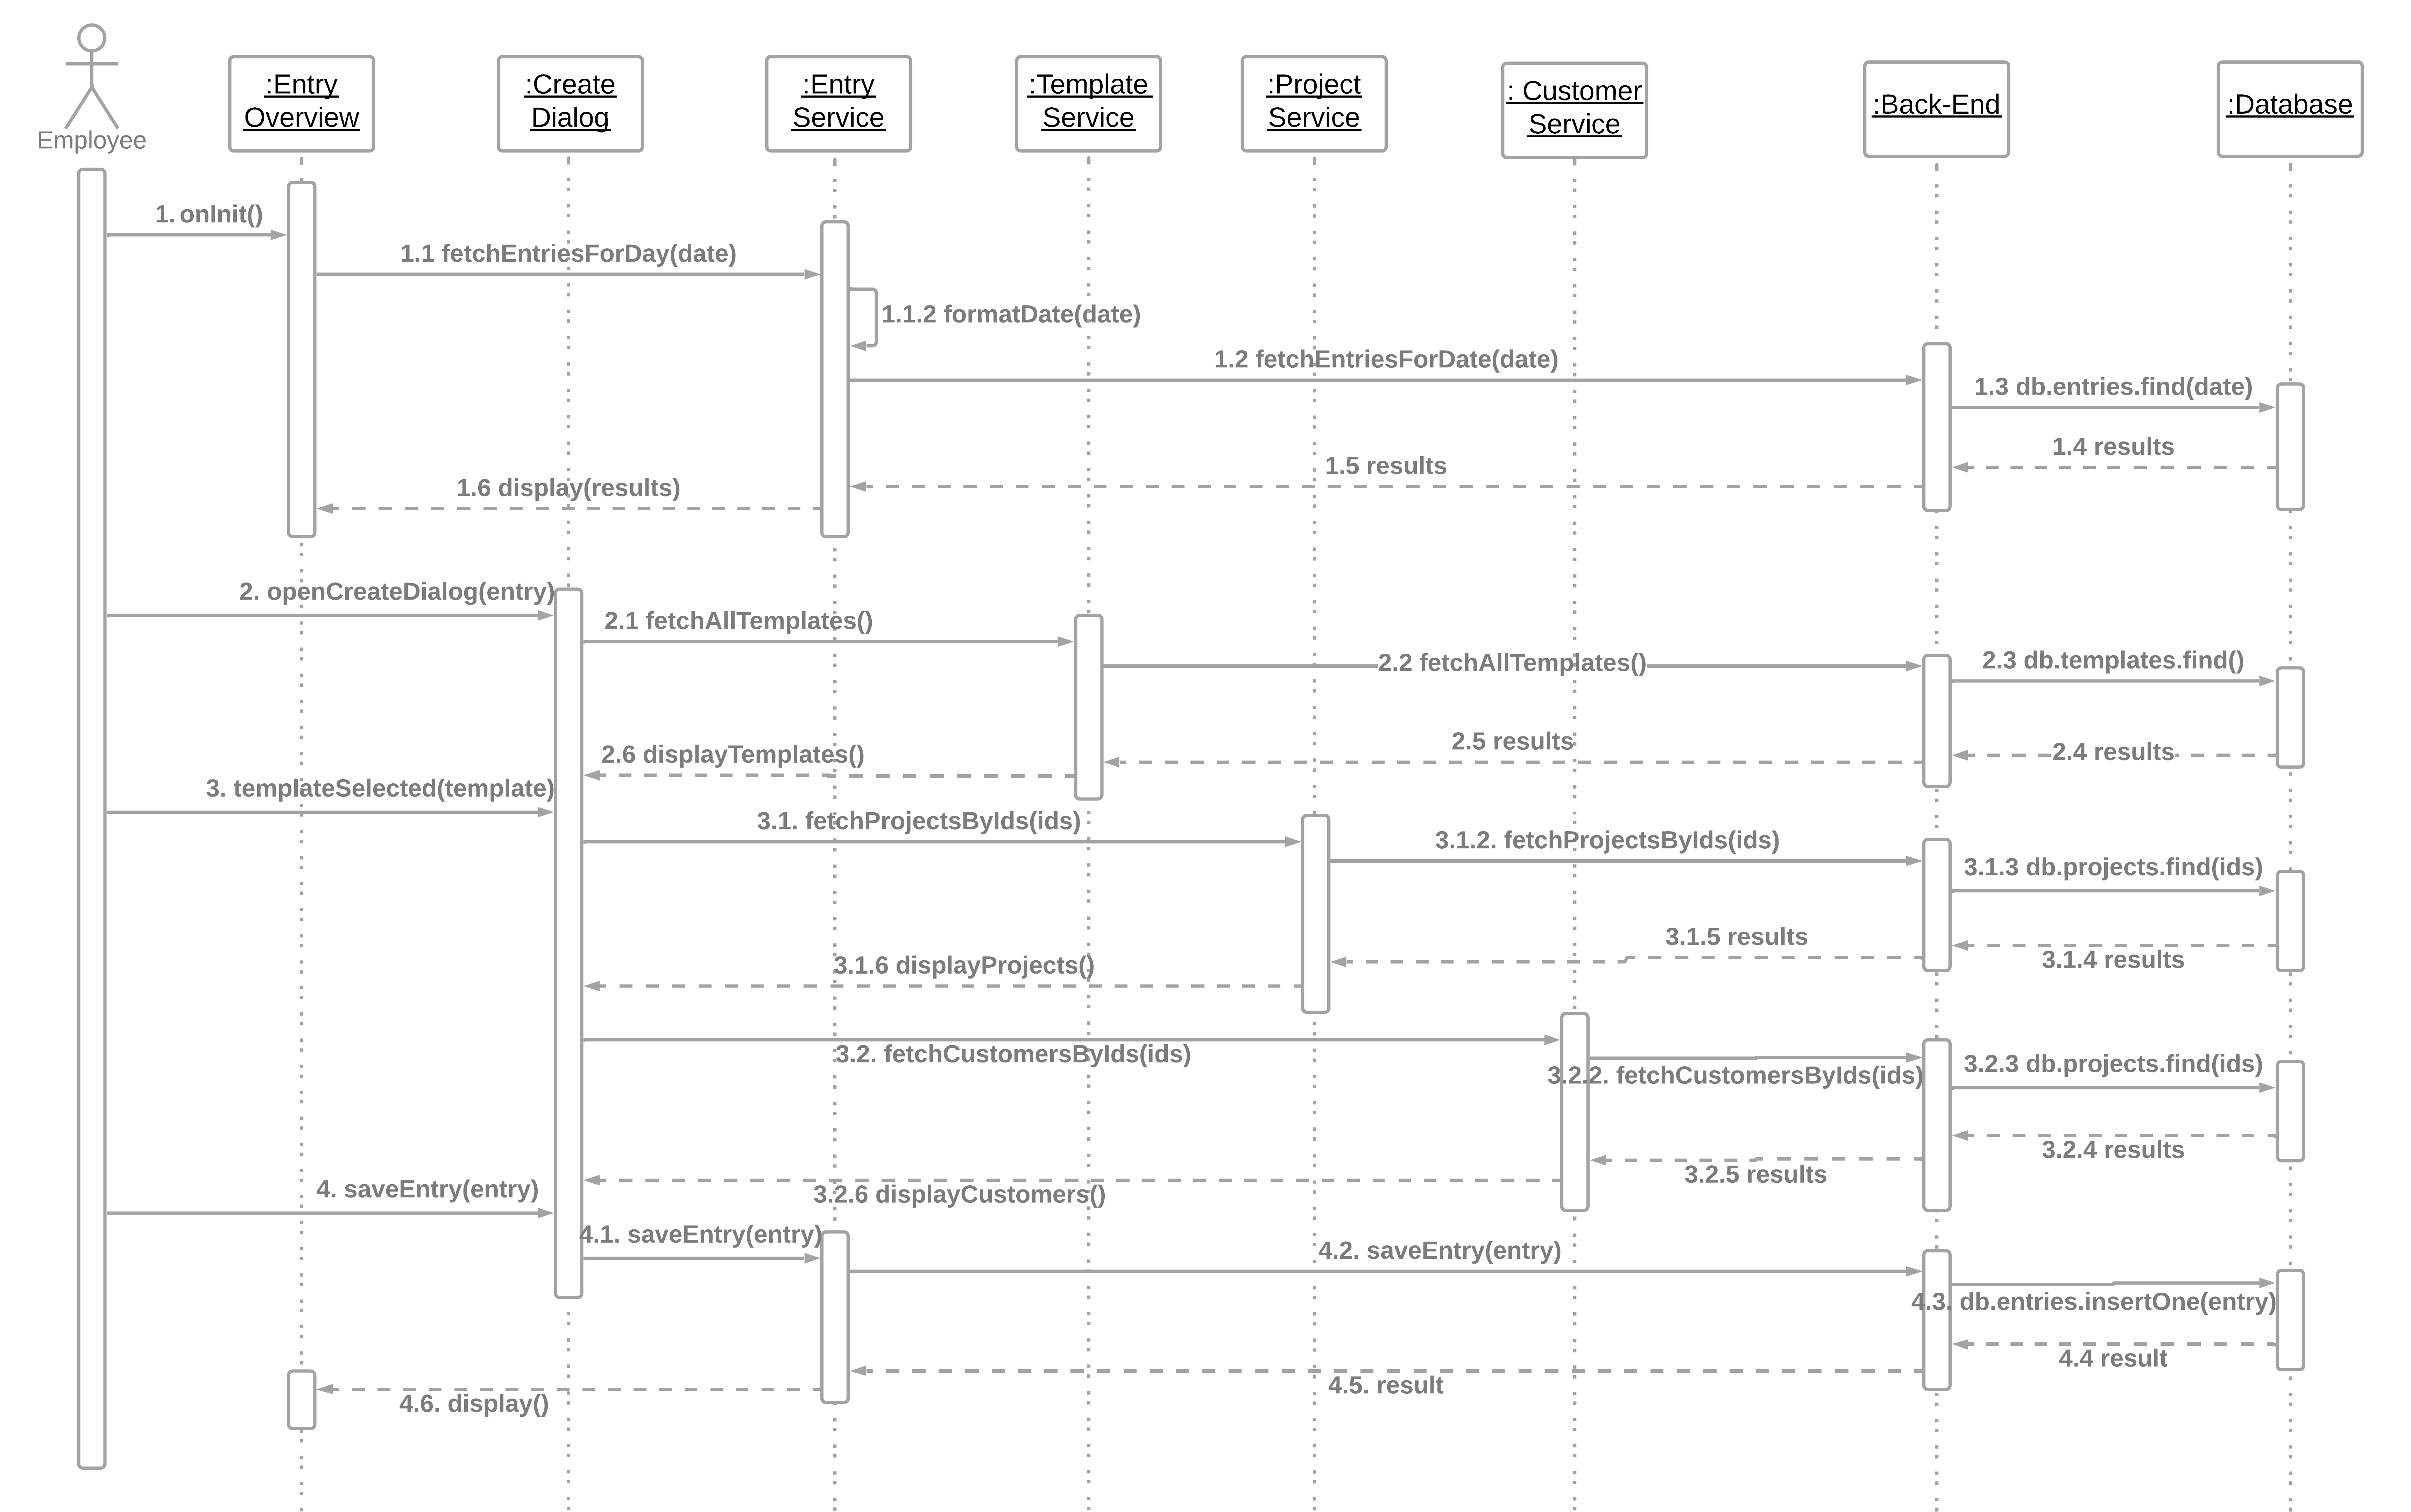
\includegraphics[width=1\textwidth]{pze-sequence-diagram}
  \caption{A sequence diagram of the Create Entry use case.}
  \label{fig:pze-sequence-diagram}
\end{figure}
After the user has started the application they will find themselves on the entry overview which lists all entries for the selected day.
This causes a request to the back-end to fetch all entries for the specified day. 
Once the user opens the create dialog all templates are fetched and displayed to the user to choose from. 
When the user chooses a template the projects and customers defined in the selected template are fetched from the back-end. 
After the user has entered all other necessary data they can save the newly created entry which sends the object to the back-end 
and persists it in the database. 
This is an illustration to show what the workflow behind user creation of an entry looks like and how 
entries, templates, projects and customers all work in accordance.
    \externaldocument{main.tex}
As previously described, the front-end component of this application is developed using Angular and Angular Material.
As these aspects are independent of Electron, the details of said implementation will be omitted, except the parts
where a direct communication between the front-end and angular takes place.\paragraph{}
During the course of this chapter a closer look will be taken on how an Electron application is to be developed.
That is to say, what the general structure should be, how it is set up and bootstrapped and finally how one can 
use Electron's functionality to cater to the needs specific to this application. 


    \subsection{Creating an Electron Application}\label{subsec:developing-with-electron-creation}
    As with any framework, installation comes first.
Electron can be simply installed using npm, the node package manager: \parencite{npm}
\begin{lstlisting}
    npm install -g electron
\end{lstlisting}
This installs Electron as a global dependency. 
The next step is to create a project directory and a package.json file for the Electron configuration, among other things. 
The entry point for any Electron application is a JavaScript file. 
In this specific case it is named app.js:
\begin{lstlisting}
{
    "name": "pze",
    "version": "1.0.0",
    "main": "app.js"
}
\end{lstlisting}
Note that the name property on line two is an abbreviation of the German term for this application:
Projektzeiterfassung, meaning project time keeping and abbreviated to PZE.


    \subsection{Electron and Angular}\label{subsec:developing-with-electron-angular}
    \externaldocument{main.tex}
As described previously the front-end in this application is a single page application developed with Angular.
This chapter describes the process of integrating Angular with Electron, which entails a few Angular-specific 
details developers need to look out for.
During the course of this chapter these details will be discussed and explained and include points such 
as how to configure Electron and Angular to work alongside, how communication between the two works, and 
how event handling between Electron and Angular functions.

    \subsubsection{Configuring Angular and Electron}\label{subsubsec:developing-with-electron-angular-config}
    \externaldocument{main.tex} 
After taking the steps to create and scaffold the Angular application, some configuration work needs to be done.
In the angular.json file the output directory needs to be set to the previously specified directory where 
Electron looks for the index.html file:
\begin{lstlisting}[caption=Angular configuration for Electron]
"options": {
    "outputPath": "dist/pze",
},
\end{lstlisting}
Another modification is required for the start scripts in the package.json file where the angular application has to be built 
and then the electron application:
\begin{lstlisting}[caption=Start scripts for Electron and Angular]
"scripts": {
        "start": "ng build --base-href ./ && electron .",
},
\end{lstlisting}
With this npm start can be executed and first ng build will be called, building the angular application after which the 
Electron start script will be called and the Electron application will be started.\paragraph{}
Now the app is up and running. 
An Electron instance will start with the Angular application running inside it. 
To speed up the development process, the Angular front-end should be developed separately. 
Not only does this lead to looser integration of Angular and Electron but when saving edits made to Angular 
developers need to restart the Electron build process which takes considerably longer than just reloading 
the Angular app. 
This means during development - and as long as the Electron part is not needed - developers should start the 
application with ng serve as changes will be adopted almost instantly whereas with Electron one needs to run the 
entire start script again.\paragraph{}

    \subsubsection{Communication between Angular and Electron}\label{subsubsec:developing-with-electron-angular-communication}
    \externaldocument{main.tex} 
For communicating between the front- and back-end Electron provides the ipcRenderer and ipcMain modules.
In the front-end part events are emitted with ipcRenderer. 
Electron offers various different ways of sending and receiving events.
The methods to listen to events on the ipcRenderer are as follows: \parencite{electronDocs}
\begin{itemize}
    \item ipcRenderer.on(channel, listener):\\
    This method listens to a channel and when a message on the corresponding 
    channel arrives, the listener is called.
    \item ipcRenderer.once(channel, listener):\\
    Acts similarly to ipcRenderer.on, but the listener is removed after the invocation
\end{itemize}
With ipcRenderer.removeListener(channel, listener) or\\
 ipcRenderer.removeAllListeners(channel) listeners can be removed.
Note that with ipcRenderer.removeAllListeners(channel) the channel parameter is optional and when omitted
all listeners get removed.
The ipcMain Event Emitter has the same methods as ipcRenderer to 
listen to events, with the only addition being ipcMain.handle(channel, listener).\paragraph{}
Similarly to receiving events, Electron offers multiple methods to send events from the ipcRenderer Event Emitter. 
Those methods include: \parencite{electronDocs}
\begin{itemize}
    \item ipcRenderer.send(channel, ...args):\\
     This methods sends an asynchronous message to ipcMain via the specified channel. 
    \item ipcRenderer.invoke(channel, ...args):\\
    This methods also sends an asynchronous message. 
    It does however expect a result and returns a Promise<any> to resolve the response.
    Note that on ipcMain handle() should be used to intercept these events.
    \item ipcRenderer.sendSync(channel, ...args):\\
     Same as ipcRenderer.send(channel, ...args) with the difference of 
    expecting a synchronous result.
    \item ipcRenderer.sendTo(webContentsId, channel, ...args):\\
    A method for sending an event directly to a specified window 
    using the webContentsId parameter.
    \item ipcRenderer.sendToHost(channel, ...args):\\
     Behaves the same as ipcRenderer.send(channel, ...args), with the 
    difference being that the event is sent to the <webview> element rather than the main process.
\end{itemize}
Having listed the options provided by Electron for inter-process communication the next step is to integrate the ipcRenderer into Angular.
For this, there are multiple solutions. 
To simplify development, developers can use an NPM module called ngx-electron developed by Thorsten Hans. \parencite{ngxElectron}
Ngx-electron makes calling Electron's API from Angular simpler for developers by exposing all methods available within Electron's
render process.
This means the above mentioned methods would all be accessible through this module. 
To include it in the Angular application one needs to import the module:
\begin{lstlisting}[caption=Importing ngx-electron's ElectronService into Angular]
import { NgModule } from '@angular/core';
import { BrowserModule } from '@angular/platform-browser';
import { HttpClientModule } from '@angular/common/http';

import { NgxElectronModule } from 'ngx-electron';
@NgModule({
  declarations: [
    AppComponent,
  ],
  imports: [
    BrowserModule,
    BrowserAnimationsModule,
    MaterialModule,
    HttpClientModule,
    NgxElectronModule,
  ],
  bootstrap: [AppComponent],
})
export class AppModule {}
\end{lstlisting}
After then importing the ElectronService class from the ngx-electron module in the necessary components 
one can send or listen to events by accessing the API:
\begin{lstlisting}[caption=Sending an event with ngx-electron]
this.electronService.ipcRenderer.send('getProjects');
\end{lstlisting}
For this solution to work there is a caveat however: 
If one tries to run this example with the latest stable Electron release (at the time of writing 17.1.0), the 
following error will be encountered:
\begin{lstlisting}[caption=Error with ngx-electron and Electron > 13.6.9]
Error: node_modules/ngx-electron/lib/electron.service.d.ts:17:31 - error TS2694: 
Namespace 'Electron.CrossProcessExports' has no exported member 'Remote'.

17     readonly remote: Electron.Remote;
                                 ~~~~~~
\end{lstlisting}
This error occurs because in version 12 of Electron, the remote module has been deprecated and in version 14
removed from Electron itself and moved to another package, @electron/remote. \parencite{electron14Blog}
This of course leads to an error because ngx-electron cannot locate the required module. 
Because the latest release of ngx-electron (version 2.1.1) happened in October of 2019, one can 
assume that this issue (which is still marked as open on GitHub as of March 2022) will not be fixed in 
the foreseeable future. \parencite{namespaceError}
What this means for developers is that if they wish to use ngx-electron, the latest usable stable release
of Electron is 13.6.9. 
While said release was last updated (at the time of writing) on February 2nd 2022, being forced to use
a deprecated feature and being locked into a specific version of any framework can pose a worry to 
many developers. \paragraph{}
As an alternative, developers can skip the use of ngx-electron and directly import the required electron module.
\begin{lstlisting}[caption=Requiring Electron in Angular]
const electron = (<any>window).require('electron');
\end{lstlisting}
Sending an event through the ipcRenderer would be very similar to the code sample above which is using 
ngx-electron:
\begin{lstlisting}[caption=Sending an event through ipcRenderer]
// Using ElectronService from ngx-electron
this.electronService.ipcRenderer.send('getProjects');

// Directly accessing ipcRenderer
electron.ipcRenderer.send('getProjects');
\end{lstlisting}
The advantage would be greater future-proofing because the use of a newer Electron stable release would
be possible.
Ultimately which solution is chosen is at the developer's discretion. 
For this proof-of-concept the ngx-electron module will be used.\paragraph{}
In figure six the flow of data is pictured when the application communicates with
the back-end.
One main goal of this application is to take advantage of Electron's arguably biggest asset over 
traditional web applications: offline functionality.
Due to the Electron back-end being developed with Node.js one can access all features available to Node.js 
which in a traditional application would not be accessible on the client's machine.
This means one can use the fact that Electron allows to read and write to the User's file system. 
It is therefore very trivial to implement storage of data on each client's machine.  
See the following sequence diagram for an overview of how data to back up is fetched from the API 
on startup.
\begin{figure}[H]
  \centering
  \label{fig:pze-sequence-diagram-electron}
  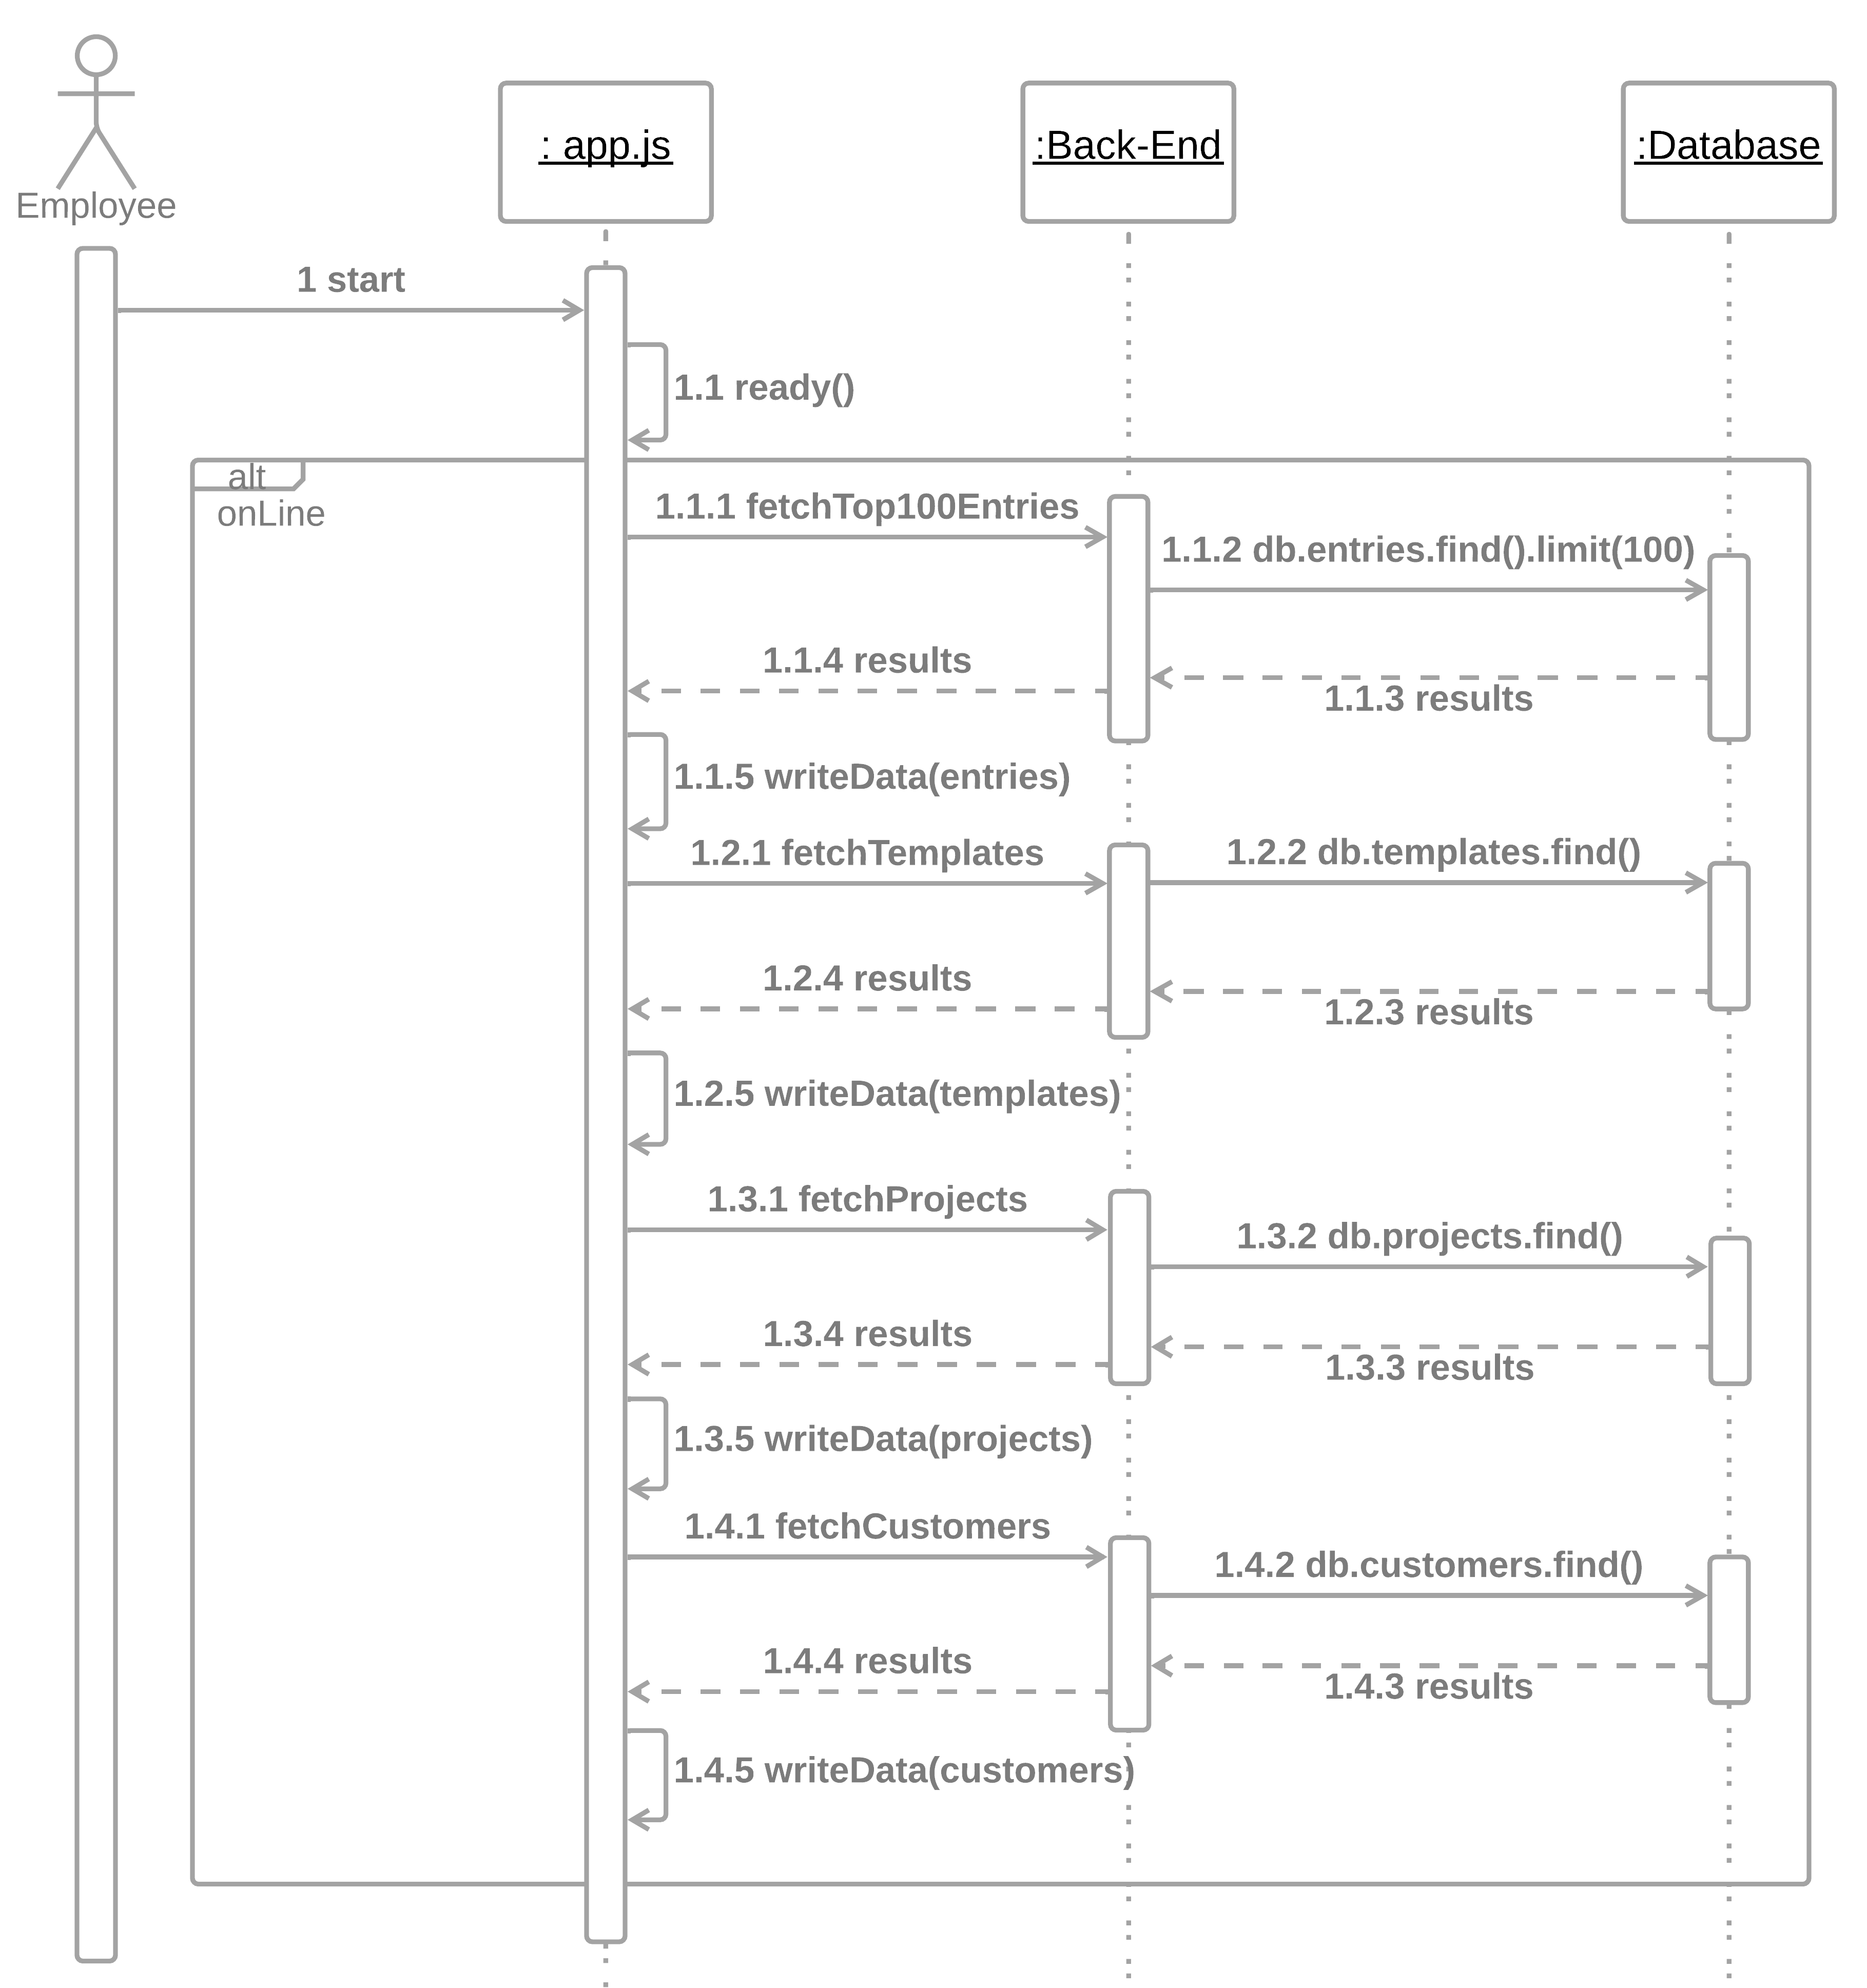
\includegraphics[width=1\textwidth]{pze-sequence-diagram-electron}
  \caption{Fetch Backup Data Sequence Diagram:
  A sequence diagram illustrating how data is fetched on startup}
\end{figure}
As pictured the API is queried if the application is online.
This is checked via the window.navigator.onLine property.
This property returns whether the client is connected to a network, be it LAN or WLAN.
The issue with this is however, that by querying whether the client is connected to a network,
the client could be connected to a network while being unable to access the internet or a specific
required resource.
Another important point about this property is the fact that browsers handle it differently.
Firefox and Internet Explorer return a false value if the browser is switched to offline or the browser
cannot establish a network connection whereas in Chrome and Safari the only case where false is returned
is when the browser cannot connect to a network. \parencite{onLineMdn}
This is to highlight another advantage of Electron: Since the browser is based on Chromium, 
developers do not need to take other browser implementations into consideration.\paragraph{}
However, as mentioned navigator.onLine is not reliable enough, because it cannot make a distinction
between no network availability or having no internet connection, let alone checking the 
host directly.
To work around this, one can send a HTTP GET request directly to the server. 
For this a /test endpoint was implemented with a 204 no content response. 
It is then trivial to send a get request and check for a 204 status.\paragraph{}
After checking whether the API is reachable, GET requests are sent to the API for the top 100 entries
and all records of project, customer and template entities. 
The returned data is then stored in corresponding JSON files as arrays. 
Note that because this is a proof-of-concept, no encryption and authentication is performed.
In a productive environment steps should be taken to only transmit data the user is authorised 
to access and ideally, stored data should be encrypted as it is stored on a client machine.\paragraph{}
After fetching data from the API to store locally the program then posts new data stored on the 
client machine to the API:
\begin{figure}[H]
  \centering
  \label{fig:pze-sequence-diagram-electron-saveNew}
  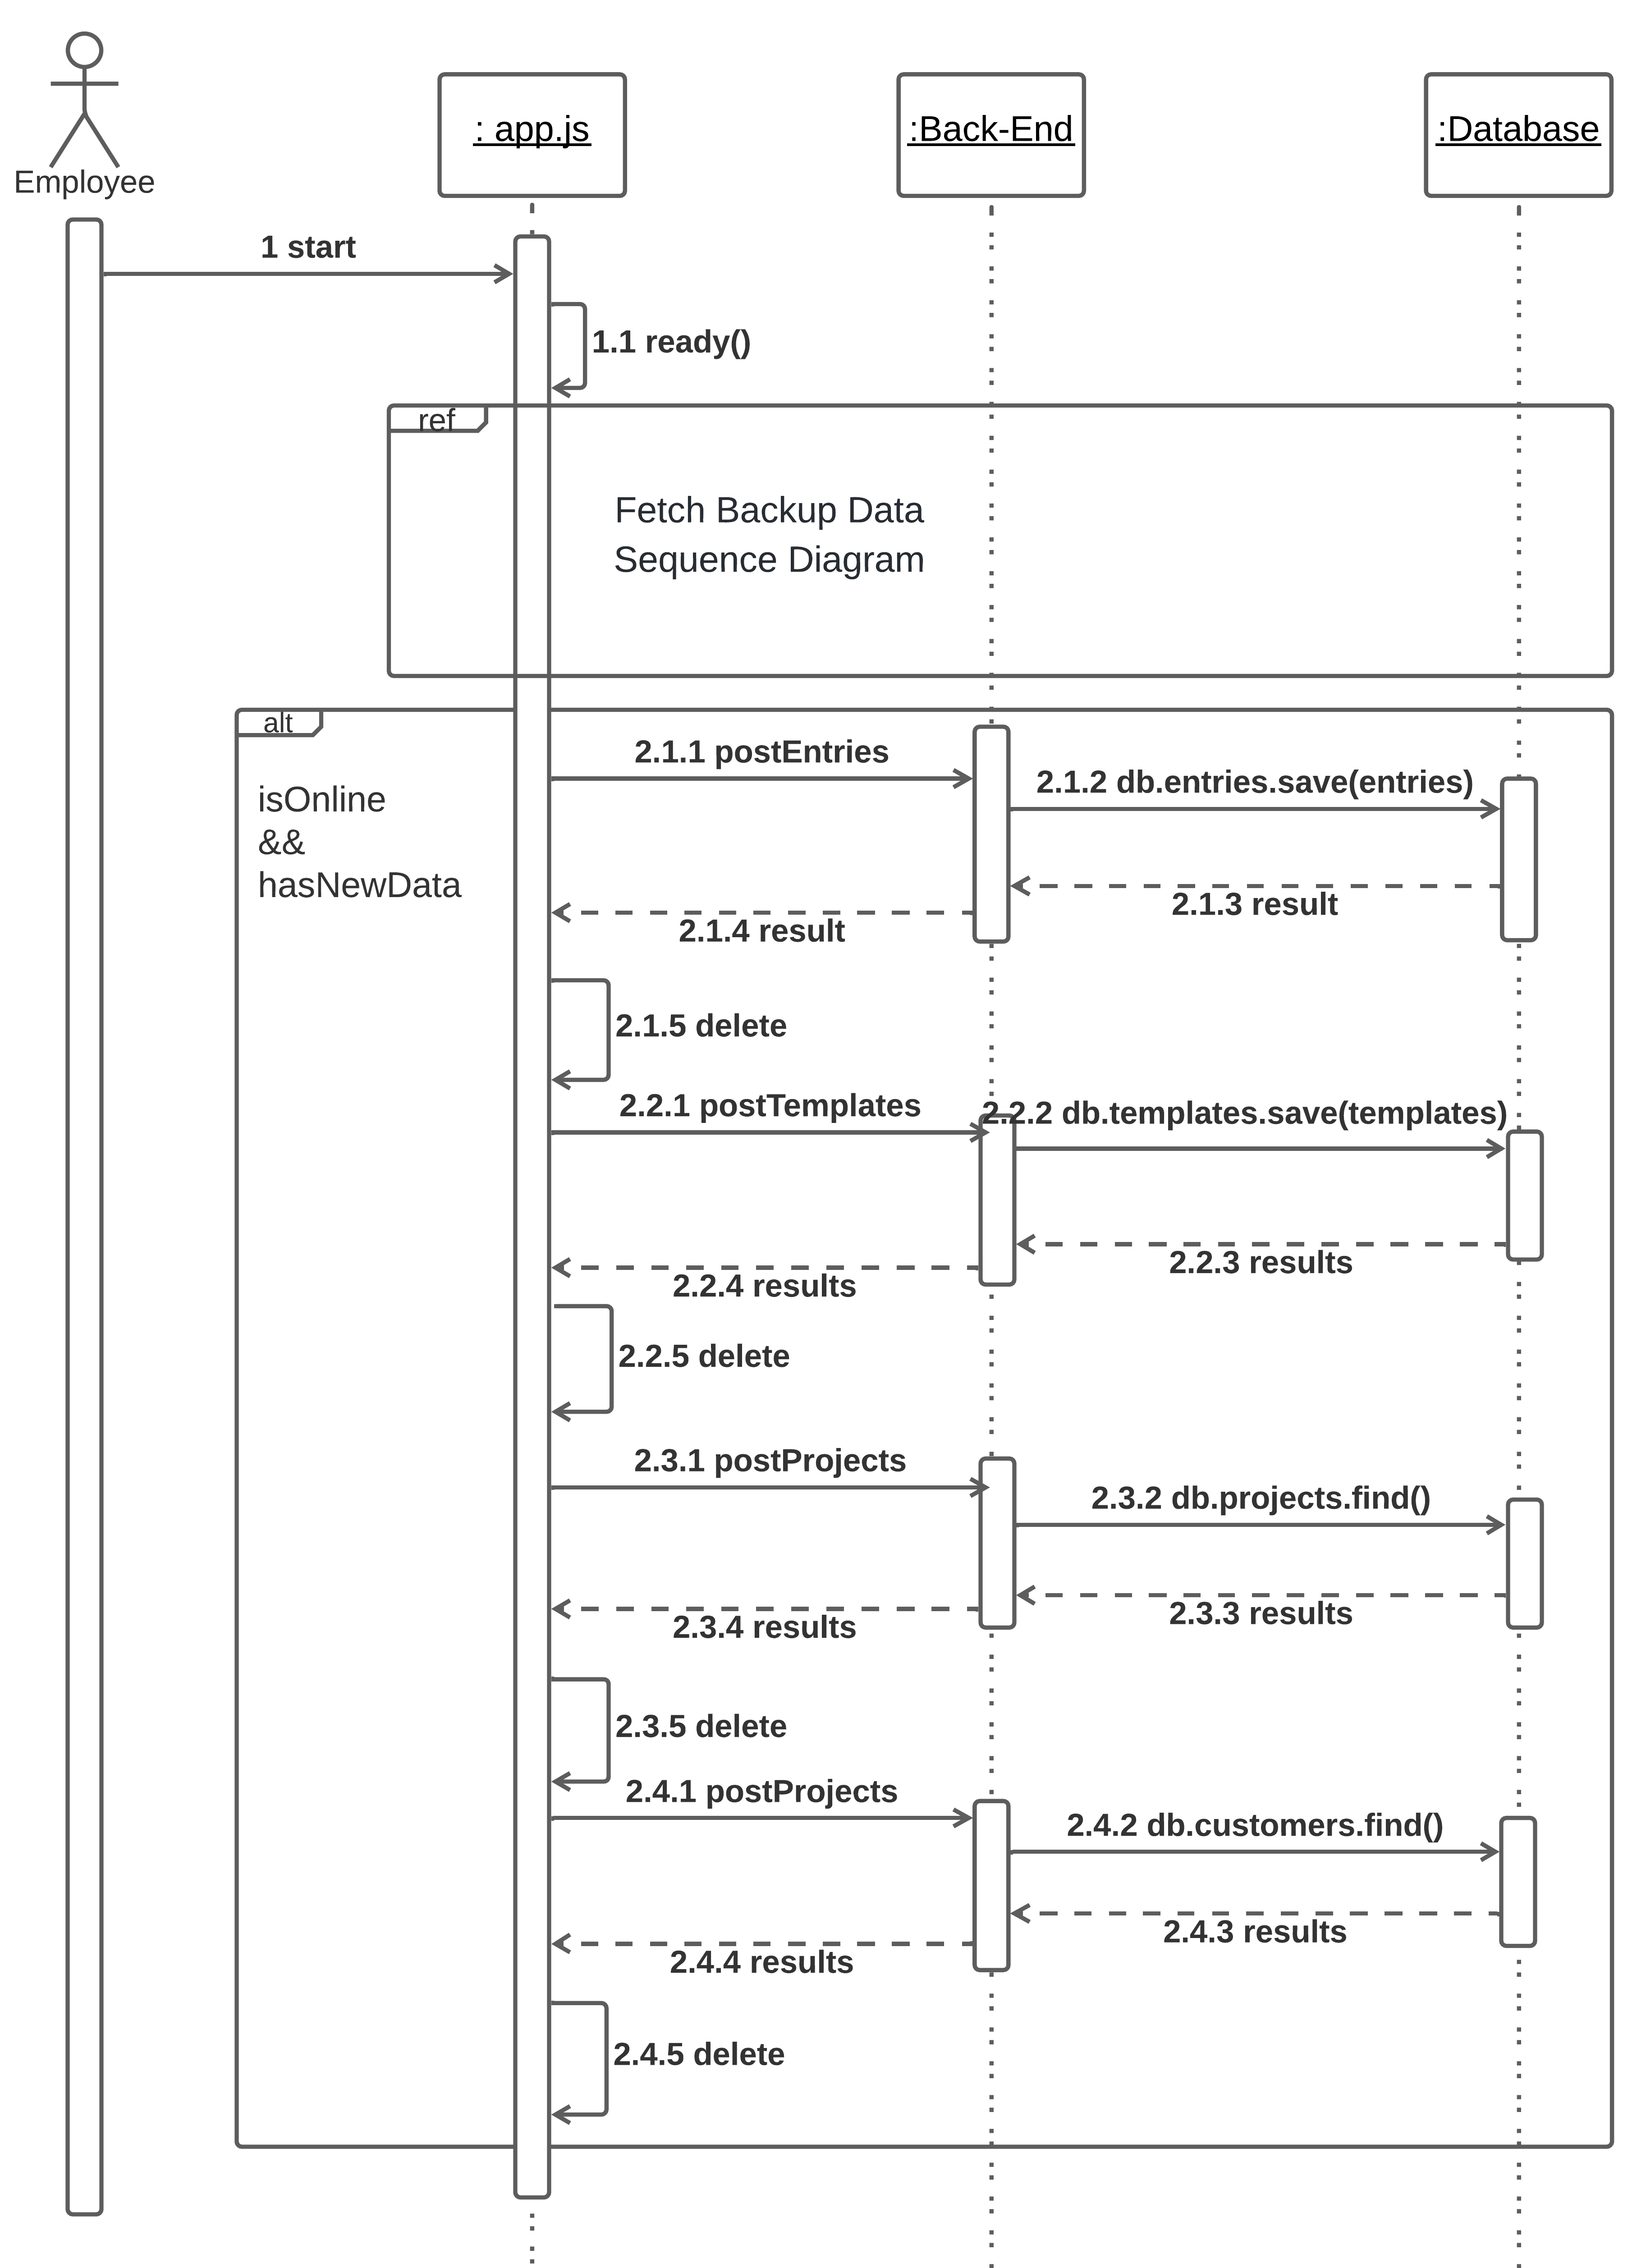
\includegraphics[width=1\textwidth]{pze-sequence-diagram-electron-saveNew}
  \caption{Post new Data to API:
  A sequence diagram illustrating how new data stored on the client machine is posted to the API}
\end{figure}
After the process outlined in figure seven, the file system is checked for new data. 
If said data exists it is then sent to the API via HTTP POST and persisted to the database.
Once this has finished the local copy of the now persisted data is deleted to avoid duplicates.\paragraph{}
Having outlined how the startup procedure for this application looks like, there is still the question of 
how one can send events and pass data between Angular and Electron.
As explained at the beginning of this chapter, ngx-electron's ElectronService will be used to send events 
to Electron from Angular. 
The process of fetching data from the Electron back-end is very similar between each entity so 
in order to illustrate the workflow see the following example of fetching customers.
\begin{lstlisting}[caption=Sending an event using ElectronService]
  this.electronService.ipcRenderer.send('getCustomers');
\end{lstlisting}
The code above emits an event called getCustomers. 
This event will be sent through the ipcRenderer EventEmitter and Electron will now listen 
for it on ipcMain.
\begin{lstlisting}[caption=Listening for an event]
  ipcMain.on("getCustomers", (event) => {
});
\end{lstlisting}
This listener will execute the callback function once it intercepts the getCustomers event. 
Within the callback function the data is read from the file system:
\begin{lstlisting}[caption=Reading data in event callback function]
  ipcMain.on("getCustomers", (event) => {
    var pathName = path.join(__dirname, `/files/pze/customers.json`);
    fs.readFile(pathName, (error, data) => {
      if (error) {
        console.error(err);
        event.reply("getCustomersReponse", null);
      } else {
        let customers = JSON.parse(data);
        let newCustomers = getNewObjects("customers_new.json");
        newCustomers.forEach(function (newCustomer) {
        customers.push(newCustomer);
      });
      console.log(customers);
      event.reply("getCustomersReponse", customers);
    }
  });
});
\end{lstlisting}
Note the use of event.reply(). 
There are a couple advantages to using event.reply(). 
Firstly, it is asynchronous. 
This means it won't block any other code from executing and one can therefore expect better performance 
than when replying with a synchronous message.
Another advantage is the fact that event.reply() automatically handles messages that originate from
different frames to the main frame. 
That is to say should the original event be fired from an iframe, this helper method will 
handle such a reply in the correct manner. \parencite{electronDocs}\paragraph{}
Currently, the application can send an event to Electron and Electron will respond with 
the requested data. 
However as of now there is no way to intercept the response and therefore data.
To achieve this there are multiple different approaches to arrive at a solution. 
One solution is to adhere to the observer pattern, a software design pattern which is used 
for event handling and asynchronous programming while handling multiple values.
In this pattern an object maintains a list of observers which are then notified by the 
subject when an event (or rather state change occurs).
Observables are widely used in Angular for the above reasons. \parencite{angularDocsObs}\paragraph{}
In order to create such an Observable which notifies its subscribers when a change occurs (in this 
case when an event from Electron is emitted), one should use the Observable<T> constructor provided
by Angular.
\begin{lstlisting}[caption=Creating an Observable for ipcRenderer]
fetchAllCustomers(): Observable<Customer[]> {
  return new Observable<Customer[]>((observer) => {
    this.electronService.ipcRenderer.on('getCustomersReponse', (event, arg) => {
      this.ngZone.run(() => {
        observer.next(arg);
      });
    });
    electron.ipcRenderer.send('getCustomers');
  });
}
\end{lstlisting}
The first step is to create an Observable, with the type parameter being an array of customers.
Following that is the call to ipcRenderer via ElectronService where a listener is created for 
the getCustomersReponse event which is the reply sent in the Electron back-end.
At the end the actual trigger event for fetching the data is sent. \paragraph{}
One important consideration is the use of NgZone. 
Zones in this context refer to persisting execution context across different asynchronous tasks.
These zones can be compared to the so-called \acrfull{tls}.
\acrshort{tls} is a method of assigning locations for data specific to a thread. \parencite{microsoftTls}
This means data is not stored globally but privately available for each thread.
Analogous to \acrshort{tls} Zones exist in JavaScript virtual machines to encapsulate 
change detection into separate execution contexts. \parencite{angularDocsZone}\paragraph{}
The underlying functionality is based on Zone.js which creates said execution contexts.
These contexts can persist asynchronous operations and Zone.js also provides lifecycle hooks 
for these asynchronous operations. \parencite{zoneJs}\paragraph{}
Angular builds on top of Zone.js with the provided NgZone service.
This service creates a zone named angular which then triggers change events when a
synchronous or asynchronous method is executed and when there is no scheduled microTask.
This separation of contexts into zones creates a problem for detecting event changes which 
happen outside of the angular zone, such is the case with Electron.
To overcome this, NgZone service offers the run() method. 
By calling this run method the code is brought back into Angular's zone and executed there 
which means change detection is carried out on all operations inside that run function. \parencite{angularDocsZone}\paragraph{}
These are the necessary steps to communicate between Angular and Electron. 
With this implementation it is trivial to pass data to Electron and return data if necessary. 
Having implemented all necessary functionality it is now time to package and deploy the Electron application.

    \clearpage

    \subsection{Using Electron's Desktop API}\label{subsec:developing-with-electron-angular-api}
    \externaldocument{main.tex}
Having described one of the advantages of Electron over web applications, namely 
extensive offline functionality, there are a lot more aspects of desktop applications
which one can access through Electron.
In this section it will be described how one can create context menus and take advantage 
of key bindings through Electron.\paragraph{}
Without specifying any menu items Electron displays basic menu options which are familiar from 
web browsers such as an edit menu with "undo" and "redo" options or a view menu in which developer
tools can be toggled among other things.
In order to create custom menu items, one must define a template in JSON form:
\begin{lstlisting}[caption=Menu template for Electron.]
const menuTemplate = [
    {
        label: "File",
        submenu: [
        {
            label: "Fetch Data",
            click: checkIfOnlineAndFetch,
        },
        {
            label: "Synchronise new Data",
            click: checkIfOnlineAndSync,
        },
        {
            label: "Toggle Offline Mode",
            click: enableOfflineMode,
        },
      ],
    },
];
\end{lstlisting}
This example creates a menu item with the label "File" and three sub menus, each of which are given 
a click handler. 
To enable this menu template Electron's Menu class offer a method named buildFromTemplate():
\begin{lstlisting}[caption=Enabling the custom menu.]
const Menu = require("electron");
const menu = Menu.buildFromTemplate(menuTemplate);
Menu.setApplicationMenu(menu);
\end{lstlisting}
The above code creates a menu from the previously defined template and then sets the now created menu
as the current application menu. 
In this case three options were added, first the option for users to manually fetch data from the API,
then the option to manually synchronise newly created, locally saved objects and finally the option
to toggle offline mode, should users wish to do so.\paragraph{}
Another useful Electron feature is the fact that key bindings can be freely chosen. 
Of course, one can also implement key bindings and combinations with regular web applications.
However, one needs to take two factors into consideration:
Key press events are handled differently across browsers and certain combinations can only be 
overridden with workarounds and arguably should not be implemented. \parencite{mdnKeyboardEvent}
For example, the \lstinline[columns=fixed]{control + N} combination is universally understood to create 
a new of something, whatever the application in question implements.
With web application, one is constrained by already existing browser key combinations, such as \lstinline[columns=fixed]{control + N} or 
\lstinline[columns=fixed]{control + T}.
For example in chrome, such an override is not possible:
\blockquote{In Chrome4, certain control key combinations [Cntr-N, Cntrl-W, Cntr-T] have been reserved for browser 
usage only and can no longer be intercepted by the client side JavaScript 
in the web page.}
\parencite{chromeIssueTrackerV4}
In addition to having to take different browsers and their versions into consideration one could also argue
that by overriding bindings such as \lstinline[columns=fixed]{control + N} one would disregard usability
conventions because users would most likely expect \lstinline[columns=fixed]{control + N} to open a new 
browser window and not something website-specific. 
As far as desktop applications go, however, one does not have to take such points into consideration.
In this example a listener on \lstinline[columns=fixed]{control + N} was added to open an edit dialog:
\begin{lstlisting}[caption=Enabling the custom menu.]
globalShortcut.register("CommandOrControl+N", () => {
    mainWindow.webContents.send("openDialog");
});
\end{lstlisting}
This creates a global shortcut for the \lstinline[columns=fixed]{control + N} or \lstinline[columns=fixed]{command + N} 
(for MacOs) combination. 
Once it is registered an event is emitted which can be intercepted in the front-end. 
Another way of adding keyboard shortcuts is to register them locally. 
That is to say these shortcuts will only trigger when the application is focused. \parencite{electronKeyboardShortcuts}
Furthermore, keyboard shortcuts can be added as so-called accelerators which means the combination will
be displayed alongside the respective option in the application menu. \paragraph{}
These are just some points Electron provides in terms of native Desktop APIs. 
Developers can leverage much more features such as notifications, Drag \& Drop, and device access among other things.
Additionally, some platform-specific APIs such as Linux launcher actions or recent documents for Windows and MacOs
exists as well.

    \subsection{Deploying an Electron Application}\label{subsec:developing-with-electron-angular-deployment}
    \externaldocument{main.tex} 
Packaging an Electron application can be carried out in two different ways which each have multiple options.
The first way is to use tooling such as electron-forge. 
The options and details with this approach will be explained later in this chapter.
The other way is to not use any tools and create a distribution manually.\paragraph{}
This can either be done by downloading the prebuilt Electron binaries and copying the 
source code into the correct location or by packaging source code into a source code archive.
The source code archive approach is beneficial in that it improves performance of file reads
on Windows. 
However, both of these approaches require additional work after the fact such as branding. \parencite{electronDocsDist}\paragraph{}
To avoid these steps it is recommended to use one of the tools available which handle packaging
the application.
These tools include electron-forge, electron-builder and electron-packager with each of them
tasked with creating the same outcome but in different ways.
In this example the application will be built with electron-packager.\paragraph{}
As mentioned previously Electron Packager is a command line tool which handles packaging 
Electron source code for distribution. 
It supports all major platforms such as Windows, Linux and MacOS which makes it trivial
for developers to create a distribution for each target platform using just one tool. \parencite{electronPackager}\paragraph{}
Electron Packager can be installed via \acrshort{npm}.
\begin{lstlisting}[caption=Installing Electron Packager]
npm install --save-dev electron-packager
\end{lstlisting}
Note that according to the project documentation it is not recommended to install the module globally. \parencite{electronPackager}
After the installation process has finished one can start building the various distributions. 
As this project was developed on a Linux machine the first distribution to be created will be a \acrfull{deb}.
The first step is to set a product name property as Electron Packager looks for such a property in the package.json file.
\begin{lstlisting}[caption=Product name property in package.json]
{
  "name": "pze",
  "productName": "PZE",
}
\end{lstlisting}
After setting the product name one can begin to build the package.
\begin{lstlisting}[caption=Command for using Electron Packager]
electron-packager . <app-name> --overwrite --asar=true --platform=<target-platform>
--arch=<x64|x86> --icon=<path/to/icon> --prune=true --out=<path/to/outDir>
\end{lstlisting}
This is the basic command for creating a build. 
The following list describes the possible values for each parameter and their meaning:
\begin{itemize}
    \item \lstinline[columns=fixed]{<app-name>} The app name specified in package.json by the name field.
    \item \lstinline[columns=fixed]{--overwrite} Optional flag for overwriting any previously created distributions.
    \item \lstinline[columns=fixed]{--asar=true} Optional flag for using asar, which is an extensive archive format
    that concatenates all files without compression.
    \item \lstinline[columns=fixed]{--platforn} The platform to build for (Windows, Linux MacOS).
    \item \lstinline[columns=fixed]{--arch} A flag for the desired architecture. 
    Can be omitted together with --platform if the --all flag (creates bundles for all
    platforms and architectures).
    \item \lstinline[columns=fixed]{--icon} Optional flag for setting the application icon.
    \item \lstinline[columns=fixed]{--prune=true} Runs the npm-prune --production command to remove all developer dependencies
    from the project.
    \item \lstinline[columns=fixed]{--out} Flag to specify the output directory.
\end{itemize}
Of course, this command can also be specified in package.json:
\begin{lstlisting}[caption=Command for Linux build specified in package.json]
"package-linux": "electron-packager . pze --overwrite --asar=true --platform=linux --arch=x64 --prune=true --out=release-builds"
\end{lstlisting}
The above example is the command for creating a package for Linux with the x64 architecture.
Once this is defined one can create the build by running \lstinline[columns=fixed]{npm package-linux}.
This process can now be repeated for each other target platform, in this case Windows and MacOS. 
Note however that a MacOS distribution can only be signed when built on a MacOS platform. \parencite{electronDocsDist}
\begin{lstlisting}[caption=Commands for Windows and MacOs builds specified in package.json]
"package-mac": "electron-packager . pze --overwrite --platform=darwin --arch=x64 --prune=true --out=release-builds",
"package-win": "electron-packager . pze --overwrite --asar=true --platform=win32 --arch=x64 --prune=true --out=release-builds",
\end{lstlisting}
After having packaged the application it is then time to create the installers. 
The first example will detail the creation of a \acrshort{deb} package. 
For this, the Electron Installer Debian is required. 
It can be installed via \acrshort{npm}:
\begin{lstlisting}[caption=Installation of electron-installer-debian]
npm install -g electron-installer-debian
\end{lstlisting}
Electron Installer Debian also requires a configuration in which certain details such as the
icon, destination and application categories are defined.
\begin{lstlisting}[caption=Configuration for debian package: debian.json]
{
    "dest": "release-builds/",
    "categories": [
        "Utility"
    ],
    "lintianOverrides": [
        "changelog-file-missing-in-native-package"
    ]
}
\end{lstlisting}
Optionally an icon can be specified, which has been omitted in this case. 
The categories field describes the type of the application such as game, science or in this case utility.
Lastly there is a property to quiet Lintian, which is a debian package checker.
The installer creation needs its own script with a few properties, which can be defined in 
package.json as well:
\begin{lstlisting}[caption=Configuration for debian package: debian.json]
"create-debian-installer": "electron-installer-debian --src release-builds/pze-linux-x64/ --arch amd64 --config debian.json"
\end{lstlisting}
The flags in this command have the following purpose:
\begin{itemize}
    \item \lstinline[columns=fixed]{src} Points to the location where the created installer should be saved.
    \item \lstinline[columns=fixed]{--arch} Defines the architecture.
    \item \lstinline[columns=fixed]{--config} Points to the required configuration file.
\end{itemize}
As the Electron Packager has already run one can now run Electron Debian Installer with 
\lstinline[columns=fixed]{npm run create-debian-installer}.
This will result in a \acrshort{deb} package which can be installed on Linux:
\begin{figure}[H]
    \centering
    \label{fig:pze-deb-package}
    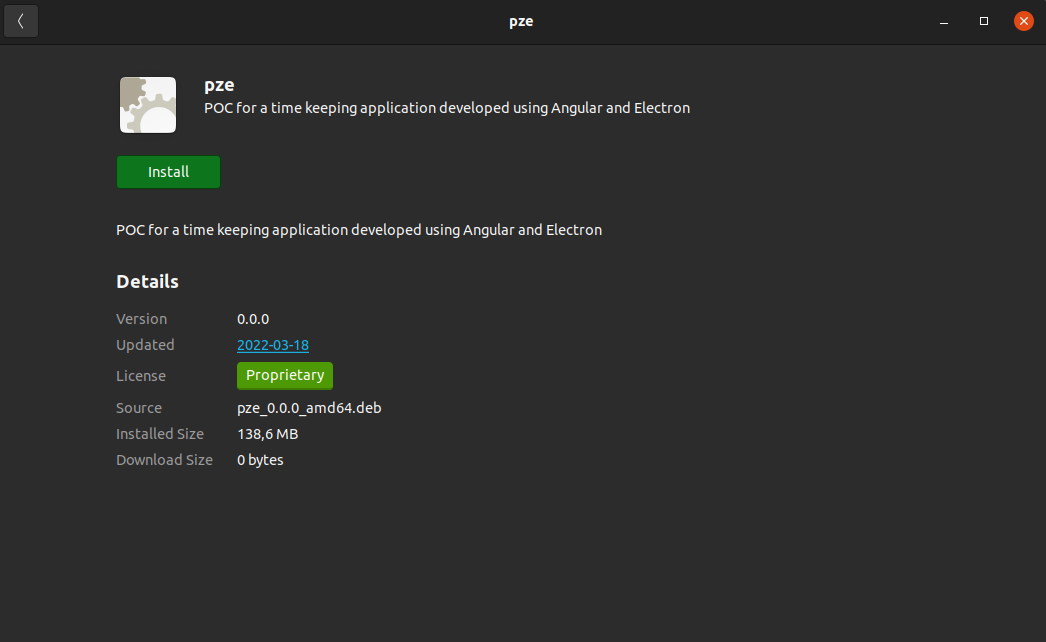
\includegraphics[width=0.8\textwidth]{deb-package}
    \caption{Installer for the recently created \acrshort{deb} package}
\end{figure}
To create a windows executable developers can choose from a number of different tools such as 
electron-installer-windows which will be used in this case.
After installing Electron Installer Windows through \acrshort{npm} as a development dependency one 
can then add the script for creating the executable:
\begin{lstlisting}[caption=Script for creating a windows executable.]
"create-win-installer": "electron-installer-windows --src release-builds/pze-win32-x64/ --dest release-builds/",
\end{lstlisting}
The parameters are analogous to those defined in the \lstinline[columns=fixed]{create-debian-installer} script.
Before execution however, one modification the the app.js file needs to be made.
More specifically, the destination of the index.html file has to be defined differently for the build process to 
work correctly. 
Currently the location of index.html is passed to the loadURL function as follows:
\begin{lstlisting}[caption=Passing index.html location to loadURL().]
mainWindow.loadURL(
    url.format({
        pathname: path.join(__dirname, `/dist/pze/index.html`),
        protocol: "file:",
        slashes: true,
    })
);
\end{lstlisting}
For the build tool to be able to correctly interpret the \_\_dirname property one needs 
to change it as such:
\begin{lstlisting}[caption=Passing index.html location to loadURL().]
mainWindow.loadURL(`file://${__dirname}/dist/pze/index.html`)
\end{lstlisting}
This means the created desktop application can then correctly load the index.html.
    \clearpage

    \section{Conclusion}\label{sec:conclusion}
    \externaldocument{main.tex}
After describing the case this chapter will now focus on answering the research questions.
As the case implementation has shown Electron is a very flexible framework 
which allows web developers to create a desktop application with very little 
additional knowledge required. 
This is arguably one of the most significant advantages of Electron which is 
also supported by the project health criterion outlined by \textcite{ratingsFW} 
which states that metrics such as the number stackoverflow.com tags correlate 
with how well known and mature a framework is. \parencite{backEndComparison}
Electron for instance has - as of April 2022 - 13525 questions tagged whereas
other competing framworks such as the briefly described NW.js is only tagged 
in 307 questions.\paragraph{}
According to \textcite{frameworksEfficiency} other evaluation criteria include
time spent developing pages, time spent modifying the existing application and size
of written code. 
As measurements in these cases have not been made, quantitative data cannot 
be provided. 
However as this case study highlights Electron in comparison to web applications
other conclusions can be drawn.
As the case study has shown the vast majority of developed code is euqivalent to 
developing a web application with a traditional client - server architecture. 
This means that Electron specific code was limited and therefore developers can 
safely assume that using Electron will not significantly increase the size of 
their written code and therefore time spent developing, debugging, testing, and
deploying. \paragraph{}
However, Electron is not without fault as has been shown by this case study.
One disadvantage is the integration of Angular into Electron has not worked flawlessly 
with some issues such as breaking changes in different versions and hard to 
degug behaviour having somewhat slowed down development. 
Another drawback of Electron which was not discussed within this case study 
is the question of security. 
As claimed by \textcite{frameworksSecurity} Electron applications often display 
security issues and vulernabilities such as cross-site-scripting or remote code execution.
Even popular and widely used applications such as Discord have had significant 
security issues in the past. \parencite{discordVulernabilities}\paragraph{}
Moving on to the benefits for users rather than developers.
As far as users go, Electron does not exhibit any disadvantages. 
For the average user it is frankly of no importance whether their application
runs in a browser or on desktop as long as their needs and wants are met which
is an area where Electron can show its strengths. 
This case study has shown developers have at least the same degree of 
design freedom in regards to user experience and user interface design 
with added benefits such as offline functionality and others as described
during this case study. 
This freedom for creativity means that developers can design their applications
in a way their users are accostumed to while also being able to create
interfaces following commonly accepted usability rules such as those
laid out by \textcite{usabilityHeuristics}.\paragraph{}
Lastly, the question of how this technology can best be used in 
a commercial environment is left to answer.
This depends on many different factors with the choice 
ultimately being at the organisation's and its 
developers' discrection. 
However, one can create certain criteria where Electron would at the 
very least be worthy of a consideration. 
As this case study has shown the only required knowledge is that 
of web development. 
That is to say that if an organisation has sufficient knowledge and 
experience in creating web applications, using Electron will require 
little if any additional training or learning. 
Another point to consider is the case which the application should serve.
Questions to ask oneself can include whether the featureset of Electron 
can be fully utilised and if Electron solves any identified problems. 
One can for example consider a simple \acrfull{crud} application within 
a business context with the purpose of managing some data. 
Electron would in this case most likely not add any additonal value 
as such basic functions can be implemented without any drawbacks with 
a classic client-server application or even other frameworks potentially better
suited for this purpose.\paragraph{}
If however offline functionality is important, the access to a client's file 
system is beneficial or even if a specific user base benefits from not having
to update their browser then Electron is at the very least worth considering.\paragraph{}
As this case study and by extension thesis can only highlight certain limited 
aspects of Electron numerous considerations for future research can be made. 
For instance an analysis of how Electron affects development time and complexity 
can be made and then analised and compared to other approaches be it desktop
or web development.
Another consideration would be how Electron fits into a productive and 
commercial environment in regards to versioning, maintenance, and further development 
which focus on any identified problem areas which could result in increased cost. 

    \clearpage

    \titleformat{\section}{\bfseries\sffamily\large\MakeUppercase}{\thesection}{0pt}{\quad}{}%
    \titlespacing{\section}{20pt}{*4}{*1.5}
    \addcontentsline{toc}{section}{Acronyms}
    \printnoidxglossary[type=\acronymtype]
    \clearpage
    \addcontentsline{toc}{section}{List of Figures}
    \listoffigures
    \clearpage
    \addcontentsline{toc}{section}{Listings}
    \counterwithin{lstlisting}{section}
    \lstlistoflistings
    \clearpage
    \addcontentsline{toc}{section}{References}
    \printbibliography
    
    


\end{document}